\chapter{Thermodynamics}
\section{Introduction to thermodynamics}
A thermodynamic system is a macroscopic system whose behaviour is identified thanks to a small and finite number of quantities - the thermodynamic properties.
\\
There is a certain degree of circularity in the definition of thermodynamic parameters, which is resolved by experiment. One considers only a restricted set of manipulations on thermodynamic systems. In practice, one allows them to be put in contact with one another, or one acts upon them by changing a few macroscopic properties such as their volume or the electric or magnetic field in which they are immersed. One then identifies a number of properties such that, if they are known before the manipulation, their values after the manipulation can be predicted. The smallest set of properties that allows one to successfully perform such a prediction can be selected as the basis for a thermodynamic description of the system.
\\ \\
If the state of a thermodynamic system can be fully characterized by the values of the thermodynamic variables, and if these values are invariant over time, one says that it is in a state of thermodynamic equilibrium. Thermodynamic equilibrium occurs when all fast processes have already occurred, while the slow ones have yet to take place. Clearly the distinction between fast and slow processes is dependent on the observation time $\tau$ that is being considered.
\\ \\
A system can be shown to be in equilibrium if the observation time is fairly short, while it is no longer possible to consider it in equilibrium for longer observation times. A more curious situation is that the same system can be considered in equilibrium, but with different properties, for different observation times.
\\ \\
Let us consider two thermodynamic systems, 1 and 2, that can be made to interact with one another. Variables like the volume $V$, the number of particles $N$, and the internal energy $U$, whose value (relative to the total system) is equal to the sum of the values they assume in the single systems, are called additive or extensive.
Strictly speaking, internal energy is not extensive, unless the interaction between 1 and 2 can be neglected.
\\ \\
\textbf{The fundamental hypothesis of thermodynamics is that it should be possible to characterize the state of a thermodynamic system by specifying the values of a certain set $(X_0, X_1, \cdots, X_r)$ of extensive variables. For example, $X_0$ could be the internal energy $U$, $X_1$ the number of particles $N$, $X_2$ the volume $V$ of the system, and so on.}
\\
The central problem of thermodynamics is that \textbf{given the initial state of equilibrium of several thermodynamic systems that are allowed to interact, determine the final thermodynamic state of equilibrium}.
\\ \\
The interaction between thermodynamic systems is usually represented by idealized walls that allow the passage of one (or more) extensive quantities from one system to the other.
Among the various possibilities, the following are usually considered:
\begin{itemize}
\item \textbf{Thermally conductive walls} These allow the passage of energy, but not of volume or particles. 
\item \textbf{ Semipermeable walls} These allow the passage of particles belonging to a given chemical species (and consequently also of energy)
\end{itemize}
The space of possible states of equilibrium (compatible with constraints and initial conditions) is called the space of virtual states. The initial state is obviously a (specific) virtual state. The central problem of thermodynamics can obviously be restated as follows:
\\
\textbf{Characterize the actual state of equilibrium among all virtual states.}

\section{Entropy formulation of thermodynamics}
\subsection{Property of entropy function}
There exists a function S of the extensive variables $(X_0, X_1, \cdots, X_r)$, called the entropy, that assumes the maximum value for a state of equilibrium among all virtual states and that possesses the following properties:
\begin{enumerate}
\item \textbf{Extensivity}: If 1 and 2 are thermodynamic systems, then 
\[ S^{(1 \cup 2)} = S^{(1)} + S^{(2)} \]
\item \textbf{Convexity}: If $ X^1 = (X_0^1, X_1^1, \cdots, X_r^1)$ and $X^2 = (X_0^2, X_1^2, \cdots, X_r^2)$ are two thermodynamic states of the same system, then for any a between 0 and 1, one obtains
\[ S[(1-\alpha)X^1 + \alpha X^2] \geq (1 - \alpha)S(X^1) + \alpha S(X^2) \]
From this expression, if we take the derivative with respect to $\alpha$ at $\alpha = 0$, we obtain
\[\left. \sum_{i=0}^{r} \frac{\partial S}{\partial X_i} \right|_{X^1} (X_i^2 - X_i^1) \geq S(X^2) - S(X^1) \]
which expresses the fact that the surface $S(X_0, X_1, \cdots, X_r)$ is always below the plane that
is tangent to each of its points. (We adpot the convention that convex means upper convex).
\item \textbf{Monotonicity}: $S(U, X_1, \cdots, X_r)$ is a monotonically increasing function of the internal energy $U$:
\[\left. \frac{\partial S}{\partial U} \right|_{X_1,\cdots,X_r} = \frac{1}{T} > 0\]
\end{enumerate}
The entropy postulate allows one to solve the central problem of thermodynamics, by referring it back to the solution of a constrained extremum problem:
\textbf{The equilibrium state corresponds to the maximum entropy compatible with the constraints.}

\subsection{Simple problems}
\subsubsection{Thermal Contact}
Let us consider two systems, 1 and 2, that are in contact by means of a thermally conductive wall. The virtual state space is therefore defined by the relations:
\[U^{(1)} + U^{(2)} = U = \mathrm{const.}\]
\[X^{(1)}_{i} = \mathrm{const}. \quad X^{(2)}_{i} = \mathrm{const.}. \quad r = 1,\cdots,r \quad \]
Let us look for the maximum of $S$ as a function of $U^{(1)}$:
\[\frac{\partial S}{\partial U^{(1)}} = \left. \frac{\partial S^{(1)}}{\partial U^{(1)}} \right|_{U^{(1)}} -  \left. \frac{\partial S^{(2)}}{\partial U^{(2)}} \right|_{U-U^{(1)}}\]
If we denote the value of $U^{(1)}$ at equilibrium by $U^{(1)}_{\mathrm{eq}}$, then we have
\[\left. \frac{\partial S^{(1)}}{\partial U^{(1)}} \right|_{U^{(1)}_{\mathrm{eq}}} =  \left. \frac{\partial S^{(2)}}{\partial U^{(2)}} \right|_{U^{(2)}_{\mathrm{eq}}}\]
Due to entropy's convexity, we can futher derive that
\[\left[ \left. \frac{\partial S^{(1)}}{\partial U^{(1)}} \right|_{U^{(1)}_{\mathrm{in}}} -  \left. \frac{\partial S^{(2)}}{\partial U^{(2)}} \right|_{U^{(2)}_{\mathrm{in}}}\right] (U^{(1)}_{\mathrm{eq}} - U^{(1)}_{\mathrm{in}}) \geq 0\]
Let us introduce the quantity
\[T = \left( \frac{\partial S}{\partial U} \right)^{-1}\]
According to our hypotheses, this quantity is positive. We obtained the following results:
\begin{itemize}
\item At equilibrium, $T$ is the same in all subsystems that are in reciprocal contact by means of thermally conductive walls.
\item In order to reach equilibrium, energy shifts from systems with higher values of $T$ toward systems with lower values of $T$.
\end{itemize}
Later, we will show that $T$ is the temperature of the system.

\subsubsection{A Thermally Conductive and Mobile Wall}
In this case, the two systems can also exchange volume $V$, in addition to internal energy $U$. If we introduce the quantity $p$ by
\[\frac{p}{T} =  \frac{\partial S}{\partial V} \]
The two equilibrium conditions are
\[T^{(1)} = T^{(2)} \quad p^{(1)} = p^{(2)}\]
One can easily prove that between two systems, both initially at the same temperature, volume is initially released by the system in which $p$ is lower to the system in which $p$ is higher. Later, we will show that $p$ is the pressure of the system.

\subsubsection{A Semipermeable Wall}
Let us consider a system composed of several chemical species, and let us introduce the number of molecules $N_1, \cdots, N_{r}$ belonging to the chemical species that constitute it as part of the thermodynamic variables. Let us suppose that two systems of this type are separated by a wall that only allows the $k$-th chemical species to pass. Clearly, it is impossible for the exchange of molecules to occur without an exchange of energy. If we introduce the quantity $\mu_i$ by
\[\frac{\mu_i}{T} =  \frac{\partial S}{\partial N_i} \]
The equilibrium conditions will therefore be
\[T^{(1)} = T^{(2)} \quad \mu^{(1)} = \mu^{(2)}\]
We will define $\mu_i$ as the chemical potential of the specie $i$.

\subsection{Heat and Work}
From mechanics (and from electromagnetism), we can derive an expression for the infinitesimal mechanical work performed on the system by varying the extensive quantities. One usually adopts a sign convention according to which work is considered positive if the system performs work on the outside. Following this convention, the expression of infinitesimal work is given by
\[\delta W  =  -\sum_{i = 1}^{r} f_i dX_i\]
On the one hand, we have
\[dS = \frac{dU}{T} + \sum_{i = 1}^{r} \left. \frac{\partial S}{\partial X_i} \right|_{U,\cdots,X_r} dX_i\]
It can be written as
\[dU = TdS - \sum_{i = 1}^{r} \left. T \frac{\partial S}{\partial X_i} \right|_{U,\cdots,X_r} dX_i\]
On the other hand, we have
\[dU = \delta Q - \delta W\]
So we can get
\[\delta Q = TdS \quad \left. \frac{\partial S}{\partial X_i} \right|_{U,\cdots,X_r} = - \frac{f_i}{T}\]

\subsubsection{Temperature}
Let us consider a system made up of a thermal engine and two heat reservoirs with $T_1 > T_2$. A heat reservoir is a system for which $T$ is independent of $U$. The whole compound system is enclosed in a container that allows it to exchange energy with the environment only in a purely mechanical way. 
\\
Let the system evolve from an initial equilibrium condition, in which the first heat reservoir has internal energy $U_1$, the second has internal energy $U_2$ , and the thermal engine is in some equilibrium state, to a final equilibrium state in which the first heat reservoir has internal energy $U'_1$, the second has $U'_2$. So $W = (U_1 + U_2 ) - (U'_1 + U'_2)$, and the thermal engine is back to its initial state. By definition, the efficiency of the engine is given by $\eta = \frac{W}{U_1 - U'_1}$.
\\
In a transformation of this kind, the total entropy of the compound system cannot become smaller. Thus, we have
\[S^{(1)}(U_1) + S^{(2)}(U_2) \leq S^{(1)}(U'_1) + S^{(2)}(U'_2)\]
On the other hand, since we are dealing with heat reservoirs, we have
\[S^{(i)}(U'_i) = S^{(i)}(U_i) + \frac{U'_i - U_i}{T_i} \quad i = 1,2\]
Thus, we have
\[\frac{U_1 - U'_1}{T_1} \leq \frac{U'_2 - U_2}{T_2}\]
Therefore,
\[\eta \leq 1 - \frac{T_2}{T_1}\]
Compared with the maximum efficiency evaluated in elementary thermodynamics, we can conclude that $T$ is the absolute temperature, up to an overall factor, which can be fixed to $1$ by rescaling the $S$. 

\subsubsection{Pressure}
Let us consider an infinitesimal variation of $V$. In this case, mechanics tells us that the work performed by the system is given by $\delta W = PdV$. So we have
\[\left. \frac{\partial S}{\partial V} \right|_{U,\cdots,X_r} = \frac{P}{T}\]
This allows us to identify the pressure $P$ with the quantity $p$ we defined previousl.


\subsubsection{The Fundamental Equation}
The equation
\[S = S(X_0 = U, X_1, \cdots, X_r)\]
is called the fundamental equation, and it represents a complete description of the thermodynamics of the system being considered.

\section{Thermodynamic potential}
\subsection{Energy Scheme}
We can also use a different (but equivalent) formulation of the fundamental principle of thermodynamics, in which entropy assumes the role of an independent variable, while energy becomes a dependent variable that satisfies a variational principle. This formalism is known as the energy scheme. In this formalism, the maximum entropy principle is replaced by the principle of minimum internal energy:
\\ 
\textbf{Among all states with a specific entropy value, the state of equilibrium is that in which internal energy is minimal.}
\\ \\
Let $\Delta X$ be a virtual variation of the extensive variables (excluding internal energy $U$) with respect to the equilibrium value $X_{\mathrm{eq}}$. Then
\[\Delta S = S(U,X_{\mathrm{eq}} + \Delta X) - S(U,X_{\mathrm{eq}} ) \leq 0\]
Since $S$ is a monotonically increasing function of $U$, there exists a value $U' > U$ such that $S(U',X_{\mathrm{eq}} + \Delta X) = S(U, X_{\mathrm{eq}})$. Therefore, if $S$ is kept constant, as the system moves out of equilibrium, $U$ cannot but increase. This is what we wanted to prove.
\\
Therefore, the fundamental equation in the energy scheme is
\[U = U(S,X_1,\cdots,X_r)\]
$U$'s differential assumes the form
\[dU = TdS + \sum_{i=1}^r f_i dX_i\]
Further more, we can derive that
\[ U[(1-\alpha)Y^1 + \alpha Y^2] \leq (1 - \alpha)U(Y^1) + \alpha U(Y^2) \]
which implies that the internal energy function is concave.

\subsection{Intensive Variables and Thermodynamic Potentials}
The derivatives $f_i = \frac{\partial U}{\partial X_i}$ of the internal energy $U$ with respect to extensive quantities $S$, $\{X_i\}$ are called intensive quantities. For uniformity's sake, we define $f_0 \equiv \frac{\partial U}{\partial X_i} = T$. A given quantity $f_i$ is called the conjugate of the corresponding variable $X_i$, and vice versa. The temperature $T$ and entropy $S$ are therefore conjugates, as are the pressure (with the opposite sign) $-P$ and the volume $V$.
\\ \\
Since both $U$ and $X_i$ are extensive, in a homogeneous system, intensive variables are not dependent on system size. Moreover, if a system is composed of several subsystems that can exchange the extensive quantity $X_i$, the corresponding intensive variable $f_i$ assumes the same value in those subsystems that are in contact at equilibrium.
\\
We now want to identify the state of equilibrium among all states that exhibit a given value of an intensive variable $f_i$. Specifically, for $i = 0$, we are confronted with the case of system with a fixed temperature, i.e. heat reservoir.
\\ \\
Let us now define the Helmholtz free energy $F(T,X) $ by the relation
\[F(T,X) = U(S(T,X),X) - TS(T,X)\]
where $X = \{ X_1,\cdots,X_r\}$.
We can then show that the thermodynamical equilibrium in these conditions is characterized by the following variational principle:
\\
\textbf{The value of the Helmholtz free energy is minimal for the equilibrium state among all virtual states at the given temperature $T$.}
\\ \\
Let us now consider more generally the Legendre transform of the internal energy $U$ with respect to the intensive variable $f_i$:
\[\Phi(S,f_1,X_2,\cdots,X_r) = U(S,X_1(S,f_1,X_2,\cdots,X_r),X_2,\cdots,X_r) - f_1 X_1 (S,f_1,X_2,\cdots,X_r)\]
where $X_1(S,f_1,X_2,\cdots,X_r),X_2,\cdots,X_r)$ is determined by the condition
\[f_1 =\left. \frac{\partial U}{\partial X_1} \right |_{S,X_2,\cdots,X_r}\]
Then, the state of equilibrium is specified by the following criterion:
\\
\textbf{Among all the states that have the same value as $f_1$, the state of equilibrium is that which corresponds to the minimum value of $\Phi$.}
\\ \\
Let us observe that the partial derivative of $\Phi$, performed with respect to $f_1$, with the other extensive variables kept fixed, yields the value of the extensive variable $X_1$:
\[ \left. \frac{\partial \Phi}{\partial f_1} \right|_{S,X_2,\cdots,X_r} = -X_1(S,f_1,X_2,\cdots,X_r)\]
\\ \\
Nothing prevents us from considering two or more intensive variables as fixed—for example, $f_0 = T$ and $f_1$. Similar considerations will then lead us to introduce the thermodynamic potential $\Phi(T,f_1,X_2,\cdots,X_r)$, obtained as a Legendre transform of $U$ with respect to $S$ and $X_1$:
\[\Phi(T,f_1,X_2,\cdots,X_r) = U - TS - f_1X_1\]
\\
This thermodynamic potential assumes at equilibrium the minimum value among all the states with the same values of $T$ and $f_1$. We can therefore obtain a whole series of thermodynamic potentials, by using a Legendre transform with respect to the extensive variables $X_i$. We cannot however eliminate all extensive variables in this manner. We will see later that if we did this, the resulting thermodynamic potential would identically vanish. For the time being, it is sufficient to observe that the $\Phi$ potentials are extensive quantities, and one cannot see how they could be a function only of intensive quantities like the $f_i$.
\\
A general thermodynamic potential
\[\Phi(S,f_1,\cdots,f_k,X_{k+1},\cdots,X_r) = U - \sum_{i = 1}^{k} f_i X_i\]
is concave as a function of the remaining extensive variables, for fixed values of the intensive variables $f_1,\cdots,f_k$.
$\Phi$ on the other hand is convex as a function of the intensive variables $f_i$s, when the extensive variables are fixed.

\subsection{Free Energy and Maxwell Relations}
The natural variables of $F$ are the temperature $T$ and the extensive variables $X_1,\cdots,X_r$, entropy excluded. Entropy can be obtained by taking the derivative of $F$ with respect to $T$. The expression for the differential of $F$ is
\[dF = -SdT + \sum_{i = 1}^{r} f_i dX_i\]
More specifically, by setting $X_1 = V$, one has
\[-P =\left. \frac{\partial F}{\partial V} \right|_{T,X_2,\cdots,X_r}\]
If we now take this equation's derivative with respect to $T$ and we use the theorem of the equality of mixed derivatives, we obtain
\[\left. -\frac{\partial P}{\partial T} \right|_{V,X_2,\cdots,X_r} = -\frac{\partial^2 F}{\partial T \partial V} = \left. -\frac{\partial S}{\partial V} \right|_{T,X_2,\cdots,X_r}\]
These relations between thermodynamic derivatives that derive from the equality of mixed derivatives of thermodynamic potentials are called Maxwell relations.
\\
The free energy designation is derived from the following property. If a system is put in contact with a reservoir at temperature $T$, we can prove the maximum quantity of work $W_{\mathrm{max}}$ that it can perform on its environment is equal to the variation in free energy between the initial and final states. In other words, one has
\[W \leq F_{\mathrm{in}} - F_{\mathrm{fin}}\]

\subsection{Gibbs Free Energy and Enthalpy}
Transforming $F$ according to Legendre with respect to $V$, we obtain a new thermodynamic potential, called the Gibbs free energy:
\[G(T,P,X_2,\cdots,X_r) = F + PV = U - TS - PV\]
The variational principle satisfied by the Gibbs free
energy is the following:
\\
\textbf{Among all states that have the same temperature and pressure values, the state of equilibrium is that in which the Gibbs free energy assumes the minimum value.}
\\
$G$'s differential is expressed as follows:
\[dG = -SdT + VdP + \sum_{i=2}^r f_i dX_i \]
We can prove that if a system is brought toward equilibrium while temperature and pressure are kept constant, the maximum work that can be performed on its environment is given precisely by the difference between the initial and final values of $G$.
\\ \\
If on the other hand, we Legendre transform the internal energy $U$ with respect to $V$, we obtain a new thermodynamic potential, usually denoted by H and called enthalpy:
\[H(S,P,X_2,\cdots,X_r) = U + PV\]
Enthalpy governs the equilibrium of adiabatic processes that occur while pressure is constant:
\\
\textbf{Among all states that have the same entropy and pressure values, the state of equilibrium is the one that corresponds to the minimum value of enthalpy.}
\\ \\
If a system relaxes toward equilibrium while the pressure is kept constant, the maximum heat that can be produced by the system is equal to its variation in enthalpy. For this reason, enthalpy it is also called free heat.
The differential of $H$ is given by
$dH = TdS + VdP + \sum_{i=2}^r f_i dX_i$
\\ \\
The equality of the mixed derivatives of $G$ and $H$ yield two more Maxwell relations:
\[\left. -\frac{\partial S}{\partial P} \right|_{T,X_2,\cdots,X_r} = \left. \frac{\partial V}{\partial T} \right|_{P,X_2,\cdots,X_r}\]

\[\left. \frac{\partial T}{\partial P} \right|_{S,X_2,\cdots,X_r} = \left. \frac{\partial V}{\partial S} \right|_{P,X_2,\cdots,X_r}\]

\subsection{Other Thermodynamic Potentials}
The Legendre transform of $F$ with respect to $N$ produces a thermodynamic potential (often written as $\Omega$) that depends on $T$, on volume $V$, on chemical potential $\mu$, and on the other extensive variables:
\[\Omega(T,V,\mu) = F - \mu N\]
Its differential is expressed as follows:
\[d\Omega = -SdT - PdV - Nd\mu\]
If one transforms $U$ instead, one obtains a rarely used potential that depends on $S$, $V$, and $\mu$, which we will designate as $\Phi$:
\[\Phi(S,V,\mu) = U - \mu N\]
Its differential is given by
\[d\Phi = TdS - PdV - Nd\mu\]
We have the following Maxwell relations
\[\left. \frac{\partial S}{\partial \mu} \right|_{T,V} = \left. \frac{\partial N}{\partial T} \right|_{\mu,V}\]
\[\left. \frac{\partial S}{\partial N} \right|_{T,V} = - \left. \frac{\partial \mu}{\partial T} \right|_{N,V}\]

\section{The Euler and Gibbs-­Duhem Equations}
\[U(\lambda S, \lambda X_1, \cdots, \lambda X_r) = \lambda U(S,X_1,\cdots,X_r)\]
By taking the derivative of this equation with respect to $\lambda$ and setting $\lambda = 1$, we obtain the Euler equation
\[TS + \sum_{i=1}^{r} f_i X_i = U\]
More particularly, for simple fluids, one obtains
\[U = TS - PV + \mu N\]
which among other things implies that
\[\mu = (U - TS + PV)/N = G/N\]
\[\Omega = U - TS - \mu N = -PV\]
More particularly, from the Euler equation, it follows that the Legendre transform of $U$ with respect to all extensive variables vanishes identically. Let us note that the interpretation of the chemical potential as a per particle density of Gibbs free energy is valid only in the case of simple fluids—in the case of a mixture of several chemical species, it is no longer valid.
If we take the Euler equation's differential, we obtain
\[dU = TdS + SdT + \sum_{i=1}^r f_idX_i + X_i df_i\]
By subtracting both sides of this equation from the usual expression of $dU$, we obtain the Gibbs-­Duhem equation:
\[SdT + \sum_{i=1}^{r}X_idf_i = 0\]
In the case of simple fluids, for example, one arrives at
\[SdT -VdP + Nd\mu = 0\]
By dividing with respect to the number of particles $N$, one obtains the Gibbs-­Duhem equation in the form
\[d\mu = vdP -sdT\]
where $v$ represents volume per particle and $s$ entropy per particle.
\\ \\
Relations between the densities and the intensive variables obtained by deriving the fundamental equation are called equations of state.
If, for example, we consider the Gibbs free energy for a simple fluid, we arrive at
\[ V = \left. \frac{\partial G}{\partial P} \right|_{T,N}\]
from which we obtain
\[v = \frac{V}{N} = v(P,T)\]
where we have made use of the fact that $G$ is extensive, and therefore proportional to $N$.
In the case of the simple fluid, we have another independent equation of state:
\[s = \frac{S}{N} = -\frac{1}{N}  \left. \frac{\partial G}{\partial T} \right|_{P}\]
which expresses the entropy per particle $s$ as a function of $P$ and $T$. In reality, the two equations of state are not completely independent, because of the Maxwell relations:
\[\left. -\frac{\partial s}{\partial P} \right|_{T} = \left. \frac{\partial v}{\partial T} \right|_{P}\]
The ideal gas is a simple fluid that satisfies the equation of state
\[P = \frac{NT}{V}\]
Maxwell relations allow us to prove that in an ideal gas, the internal energy only depends on $N$ and $T$ (and not on the volume $V$). Moreover, entropy is the sum of a term that depends only on $T$ with one that depends only
on $V$.

\section{Thermodynamic systems with multi-components}
\subsection{Chemical Reactions}
Let us now consider a mixture of $r$ chemical species, $A_1,\cdots,A_r$ , which can be transformed into one other by a reaction of the following type:
\[\nu_1A_1+\cdots+\nu_kA_k \leftrightarrows \nu_{k+1}A_{k+1}+\cdots+\nu_rA_r\]
We can conventionally assign negative stoichiometric coefficients to the products, so as to write this formula as a formal equation:
\[\sum_{i=1}^r \nu_iA_i = 0\]
If temperature and pressure are kept fixed, we can calculate the variation of Gibbs free energy for a certain variation in the number of particles due to the reaction
\[\delta G = \sum_i \left. \frac{\partial G}{\partial N_i} \right|_{P,T} \delta N_i \propto \sum_i \left. \frac{\partial G}{\partial N_i} \right|_{P,T} \nu_i = \sum_{i} \mu_i\nu_i\]
Since at equilibrium one must have $\delta G = 0$ for any virtual variation of the $N_i$, one will have
\[\sum_{i} \mu_i\nu_i = 0\]
where the stoichiometric coefficients $\nu_i$ are taken with their corresponding signs.

\subsection{Phase Coexistence}
It frequently happens that two systems characterized by different thermodynamic density values can maintain thermodynamic equilibrium even in the absence of constraints on the mutual exchange of extensive quantities. This situation is called phase coexistence.
\\
In the case of a simple fluid, it is realized, for example, when a liquid coexists with its vapor inside a container. In this case, the intensive variables assume the same value in both systems, while densities assume different values. In these cases, we refer to each of the coexisting homogeneous systems as a phase.
\\
One can describe phase coexistence by saying that the equation of state
\[v = v(P,T)\]
does not admit of a unique solution, but instead allows for at least the two solutions $v = v_{\mathrm{liq}}$ and $v = v_{\mathrm{vap}}$ which correspond to the liquid and vapor, respectively.
\\
Since the liquid and vapor coexist and can exchange particles, the chemical potential of the liquid has to be equal to that of the vapor:
\[\mu_{\mathrm{liq}}(P,T) = \mu_{\mathrm{vap}}(P,T)\]
On the other hand, we know that for a simple fluid, the chemical potential is equal to the Gibbs free energy per particle. We can verify that the Gibbs free energy in the total system does not depend on the number of particles that make up the liquid and the vapor system:
\[G= G_{\mathrm{liq}} + G_{\mathrm{vap}} = N_{\mathrm{liq}}\mu_{\mathrm{liq}} + N_{\mathrm{vap}}\mu_{\mathrm{vap}} = (N_{\mathrm{liq}}+N_{\mathrm{vap}})\mu = N\mu\]
The volume per particle of the system is given by
\[v = \frac{V_{\mathrm{liq}}+V_{\mathrm{vap}}}{N} = \frac{N_{\mathrm{liq}}v_{\mathrm{liq}} + N_{\mathrm{vap}}v_{\mathrm{vap}}}{N} = x_{\mathrm{liq}}v_{\mathrm{liq}}+x_{\mathrm{vap}}v_{\mathrm{vap}}\]
where $x_{\mathrm{liq}}$ is the fraction of particles in the liquid and $x_{\mathrm{vap}} = 1 - x_{\mathrm{liq}}$ that of the particles in the vapor. As a consequence, the value of $v$ lies somewhere between $v_{\mathrm{liq}}$ and $v_{\mathrm{vap}}$.

\subsection{The Clausius-­Clapeyron Equation}
If we consider a thermodynamic system as a function of its intensive variables, we can identify some regions in which the thermodynamic properties vary regularly with variations of their values. These regions represent thermodynamically stable phases and are limited by curves that represent phase transitions. The phase transitions can be discontinuous, like the phase coexistence we just discussed, or continuous. In the first case, the densities present a discontinuity at the transition, while in the second, they vary with continuity, even though their derivatives can exhibit some singularities. One often also employs the following terminology: discontinuous transitions are called first order transitions, while continuous ones are called second order transitions.
\\
In the case of a simple fluid, it is possible to identify the transition curve within the plane of the intensive variables $(P,T)$ - in other words, the curve $P= P_t(T)$ - from the condition of equality of the chemical potential $\mu$ between the two coexisting phases:
\[\mu_{\mathrm{liq}}(P_t(T),T) = \mu_{\mathrm{vap}}(P_t(T),T)\]
The pressure $P_t(T)$ at which the transition occurs is also called vapor pressure. It is possible to relate this curve locally with the discontinuity of densities at transition. To obtain this relation, let us take the total derivative of this equation with respect to $T$, along the transition line $P_t(T)$. We obtain
\[\left. \frac{\partial \mu_{\mathrm{liq}}}{\partial P} \right|_{T} \frac{dP_t}{dT} + \left. \frac{\partial \mu_{\mathrm{liq}}}{\partial T} \right|_{P} = \left. \frac{\partial \mu_{\mathrm{vap}}}{\partial P} \right|_{T} \frac{dP_t}{dT} + \left. \frac{\partial \mu_{\mathrm{vap}}}{\partial T} \right|_{P}\]
Therefore,
\[\frac{dP_t}{dT} = \frac{s_{\mathrm{vap}}-s_{\mathrm{liq}}}{v_{\mathrm{vap}}-v_{\mathrm{liq}}}\]
This equation, which can be applied to each case of phase coexistence, is called the Clausius - Clapeyron equation.

\subsection{The Coexistence Curve}
We can represent the phase diagram in the plane $(v,T)$, in which the intensive variable $T$ is accompanied by the density $v$, the volume per particle. In this manner, phase coexistence is represented by the existence of a forbidden region $v_{\mathrm{liq}}(T) < v < v_{\mathrm{vap}}(T)$ in the plane. Outside this region, it is possible to obtain any given value of $v$ in a homogeneous system. Within this region, instead, the system separates into a liquid and a vapor phase. The $x_{\mathrm{liq}}$ fraction of particles in the liquid phase (and the analogous fraction in the vapor phase) are determined by the condition that the entire system's volume per particle be equal to $v$. One thus obtains
\[x_{\mathrm{liq}} = \frac{v_{\mathrm{vap}}-v}{v_{\mathrm{vap}}-v_{\mathrm{liq}}}\]
This result is known as the lever rule.

\subsection{Coexistence of Several Phases}
Let us now consider a mixture of particles belonging to $r$ different chemical species. Let us suppose that we are looking for the coexistence of $q$ phases. At equilibrium, all the intensive variables must assume the same value in the coexisting phases. We will therefore have a specific value for the pressure and the temperature, and in addition the chemical potential of each species will have to assume the same value in all the different phases. If we denote the chemical potential of species $i$ in phase $\alpha$ as $\mu_i^{\alpha}$ , we will then have
\[\mu_{i}^{\alpha} = \mu_i \quad i = 1,\cdots,r \quad \alpha = 1,\cdots,\]
In this equation, $\mu_i$ is the shared value taken by the chemical potential of species $i$. We
thus obtain $r(q-1)$ equations for $q(r-1)+2$ unknown values. These unknown values are $P$, $T$, and the $q(r-1)$ independent densities $x_i^{\alpha}$ of species $i$ in phase $\alpha$. Generically speaking, therefore, $f = 2 - q + r$ free parameters remain. For $f = 0$, coexistence will occur in isolated points of the phase diagram, for $f = 1$, along a line, and so on. The quantity $f$ is called variance.  It is called the Gibbs phase rule.

\subsection{The Critical Point}
Let us once again consider the simple fluid and observe that the coexistence of liquid and vapour cannot be obtained for temperatures higher than a certain temperature $T_c$, called the critical temperature. To be more precise, the transition curve ends at a point $(P_c,T_c)$, where $P_c$ is the critical pressure. For $T < T_c$, the difference $v_{\mathrm{vap}}-v_{\mathrm{liq}}$ tends continuously toward zero when $T$ gets close to $T_c$ - the discontinuity of thermodynamic densities tends to vanish, or in other words, the transition goes from being discontinuous to being continuous (and finally to disappear at higher temperatures).
\\
The critical point is a thermodynamic state with exceptional properties. For example, since for $T < T_c$ and $P = P_t(T)$ one gets $\partial P / \partial V |_{T} = 0$ (within the coexistence curve), this relation must ultimately be valid also at the critical point - in other words, the system's compressibility diverges:
\[\chi = - \frac{1}{V} \left. \frac{\partial V}{\partial P} \right|_{T} \to \infty \mbox{ for } T \to T_c \]
Various thermodynamic properties exhibit analogous singularities.

\chapter{Principles of Statistical Mechanics and Ensembles}
\section{Density matrix}
In quantum mechanics, the state of a system is a vector in Hilbert space, denoted as $|\psi\rangle$. A physical observable is an operator on this Hilbert space, denoted as $O$. The expectation value of the measurement of the observable is $\langle \psi | O | \psi \rangle$. It is easy to verify that
\[\langle \psi | O | \psi \rangle = \mathrm{Tr}(| \psi \rangle \langle \psi | O)\]
Now, consider a system whose space of states is the direct product of two subspace, i.e.
\[\mathcal{H} = \mathcal{H}_A \otimes \mathcal{H}_B\]
An arbitrary state can be decomposed as
\[|\psi\rangle = C_{iI}|i\rangle_A \otimes |I\rangle_B\]
So, we have
\[| \psi \rangle \langle \psi | = C_{iI}C^*_{jJ} |i,I\rangle \langle j,J |\]
We define the partial trace of $| \psi \rangle \langle \psi |$ on B as
\[\mathrm{Tr}_B (| \psi \rangle \langle \psi |) \equiv \sum_{I} C_{iI}C^*_{jI} |i\rangle \langle j |\]
It is an operator on $\mathcal{H}_A$. 
Now, suppose there is an observable which measures only on A, i.e.
\[\langle i,I | O | j,I \rangle = \delta_{IJ} \langle i | O_A | j \rangle\]
where $O_A$ is an operator on $\mathcal{H}_A$. We can verify that
\[\langle \psi | O | \psi \rangle = \mathrm{Tr}(| \psi \rangle \langle \psi | O) = \mathrm{Tr}_A \left[\mathrm{Tr}_B (| \psi \rangle \langle \psi |) O_A   \right]\]
Now, if we take A as the system and B the environment, a piratical observable measures only on system. For any system which is coupled to environment, its state can be described by an operator
\[\rho = \mathrm{Tr}_{\mathrm{env}} (| \psi \rangle \langle \psi |)\]
So the expectation value of the measurement on the system is
\[\mathrm{Tr}[\rho O_{\mathrm{sys}}]\]
We can verify that
\[\mathrm{Tr}\rho = 1 ,\quad \rho^{\dagger} = \rho\]
and any eigenvalue of $\rho$ must lie between $0$ and $1$. 
Suppose $rho$ can be diagonalized as
\[\rho = \sum_i p_i |i\rangle\langle i |\]
We have
\[\mathrm{Tr}[\rho O] = p_i \langle i | O | i \rangle\]
So it is reasonable to assume $p_i$ as the (classical) probability of the system in (pure) state $|i\rangle$.
One fundamental postulate of statistical mechanics is that the entropy operator of the system is
\[\hat{S} = -\ln \rho\]
So, the expectation value of entropy is
\[S = \mathrm{Tr}[-\rho\ln\rho]\]

\section{Statistical ensemble}
\subsection{Micro-canonical ensemble}
Micro-canonical ensemble describes a system which is weakly coupled to the environment. The volume $V$ and the number of the particles $N$ are fixed. The energy of the system lies in a narrow range between $E-\Delta E$ and $E + \Delta E$. The total number of distinct microstates accessible to a system is then denoted by the symbol $\Gamma(V,N,E;\Delta)$ and, by assumption, any one of these microstates is as likely to occur as any other. 
\\
Accordingly, the density matrix in the energy representation will be of the form
\[\rho_{mn} = \rho_m \delta_{mn}\]
with
\[\rho_n = \begin{cases} 1/\Gamma \mbox{ for each of the accessible states} \\ 0 \mbox{ for all other states} \end{cases}\]
The entropy of the system is
\[S = \ln \Gamma\]

\subsection{Canonical ensemble}
Canonical ensemble describes a system which can exchange energy with the environment. The density matrix of the system is
\[\rho = \frac{e^{-\beta H}}{\mathrm{Tr}[e^{-\beta H}]}\]
Now, we define
\[Z(\beta,V,N) \equiv \mathrm{Tr}[e^{-\beta H}] \quad F(\beta,V,N) \equiv -\ln Z/\beta\]
The energy of the system is
\[U = \mathrm{Tr}[\rho H] = -\left. \frac{\partial \ln Z}{\partial \beta} \right|_{V,N}\]
If we further define $T \equiv 1/\beta$, we have
\[U = F - T \left. \frac{\partial F}{\partial T} \right|_{V,N}\]
The entropy of the system is
\[S = \mathrm{Tr}[-\rho\ln\rho] = \frac{U-F}{T}\]
We can further derive that
\[\left. \frac{\partial U}{\partial S}\right|_{V,N} = T\]
Now, we can identify $T$ as the absolute temperature and $F$ as free energy in thermodynamics.

\subsection{Grand-canonical ensemble}
Grand canonical ensemble describes a system which can exchange energy and particles with the environment. The density matrix of the system is
\[\rho = \frac{e^{-\beta (H - \mu N)}}{\mathrm{Tr}[e^{-\beta (H - \mu N)}]}\]
Now, we define
\[Z_{\Omega}(\beta,V,\mu) \equiv \mathrm{Tr}[e^{-\beta (H-\mu N)}] \quad \Omega(\beta,V,N) \equiv -\ln Z_{\Omega}/\beta\]
The particle number of the system is
\[N = \mathrm{Tr}[\rho N] = \frac{1}{\beta}\left. \frac{\partial \ln Z_{\Omega}}{\partial \mu} \right|_{V,\beta} = -\left. \frac{\partial \Omega}{\partial \mu} \right|_{V,T}\]
We also have
\[U - \mu N = -\left. \frac{\partial \ln Z_{\Omega}}{\partial \beta} \right|_{V,\mu} = \Omega - T\left. \frac{\partial \Omega}{\partial T} \right|_{V,\mu} \]
The entropy of the system is
\[S = \mathrm{Tr}[-\rho\ln\rho] = \frac{U-\mu N - \Omega}{T}\]
We can further derive that
\[\left. \frac{\partial U}{\partial N}\right|_{V,S} = \mu\]
Now, we can identify $\mu$ as the chemical potential and $\Omega$ as grand canonical potential in thermodynamics.

\section{Fluctuations}
\subsection{Canonical Ensemble}
The density matrix for canonical ensemble is
\[\rho = \frac{e^{-\beta H}}{\mathrm{Tr}[e^{-\beta H}]}\]
We have
\[\left. \frac{\partial \rho}{\partial \beta} \right|_{N,V} = -\rho H + \rho \mathrm{Tr}[\rho H]\]
Since $U = \mathrm{Tr}[\rho H]$, we can derive that
\[\left. \frac{\partial U}{\partial \beta} \right|_{N,V} = -\mathrm{Tr}[\rho H^2] + (\mathrm{Tr}[\rho H])^2 = -\langle E^2 \rangle + \langle E \rangle^2 = -\langle (\Delta E)^2 \rangle\]
So, the relative fluctuation of energy in canonical ensemble is
\[\frac{\sqrt{\langle (\Delta E)^2 \rangle}}{\langle E \rangle} = \frac{T}{U}\sqrt{\left. \frac{\partial U}{\partial T} \right|_{N,V}} = T \frac{\sqrt{C_V}}{T} \sim O(N^{-1/2})\]
For large $N$ (which is true for every statistical system) the relative r.m.s. fluctuation in the values of $E$ is quite negligible.

\subsection{Grand canonical ensemble}
Density and energy fluctuations in the grand canonical ensemble is much more complicated. The detailed discussion can be found in section 4.5 of \emph{Statistical Mechanics (R.K.Pathria \& Paul D.Beale)}. 
\\
The density fluctuation is
\[\frac{\langle (\Delta n)^2 \rangle}{\langle n \rangle^2} = \frac{T}{V}\kappa_T\]
where $ n = \frac{N}{V}$ is the number density and $\kappa_T = -\frac{1}{v} \left. \frac{\partial v}{\partial P} \right|_{T}$ is the isothermal compressibility of the system.
\\ \\
Thus, the relative root-mean-square fluctuation in the particle density of the given system is ordinarily $O(N^{-1/2})$ and, hence, negligible. However, there are exceptions, like the ones met with in situations accompanying phase transitions. In those situations, the compressibility of a given system can become excessively large, as is evidenced by an almost "flattening" of the isotherms. In the region of phase transitions, especially at the critical points, we encounter unusually large fluctuations in the particle density of the system. Such fluctuations indeed exist and account for phenomena like critical opalescence. It is clear that under these circumstances the formalism of the grand canonical ensemble could, in principle, lead to results that are not necessarily identical to the ones following from the corresponding canonical ensemble. In such cases, it is the formalism of the grand canonical ensemble that will have to be preferred because only this one will provide a correct picture of the actual physical situation.
\\ \\
The energy fluctuation in grand canonical ensemble is 
\[\langle (\Delta E)^2 \rangle = T^2C_V + \left(\left. \frac{\partial U}{\partial N} \right|_{T,V} \right)^2 \langle (\Delta N)^2 \rangle\]
The mean-square fluctuation in the energy of a system in the grand canonical ensemble is equal to the value it would have in the canonical ensemble plus a contribution arising from the fact that now the particle number $N$ is also fluctuating. Again, under ordinary circumstances, the relative root-mean-square fluctuation in the energy density of the system would be practically negligible. However, in the region of phase transitions, unusually large fluctuations in the value of this variable can arise by virtue of the second term in the formula.

\chapter{Interaction-free Systems}
\section{General discussion}
\subsection{Bose-Einstein Statistics}
If the system is composed of interaction-free Bosons, the state of the system can be denoted as
\[|n_1,n_2,\cdots,n_i,\cdots\rangle\]
where $n_i$ is the number of particles in state $|i\rangle$. Here, we choose $|i\rangle$ to the energy eigenstate with energy $\epsilon_i$. 
\\
If we adopt grand-canonical ensemble, we have
\[Z_{\Omega} = \mathrm{Tr}[e^{-\beta(H-\mu N)}] = \sum_{n_1,\cdots,n_i,\cdots} e^{-\beta \sum_{i}n_i(\epsilon_i-\mu)} = \prod_{i}\sum_{n_i=0}^{\infty}[e^{-\beta(\epsilon_i-\mu)}]^{n_i} = \prod_{i} \frac{1}{1-e^{-\beta(\epsilon_i - \mu)}}\]
So, the grand canonical potential of the system is
\[\Omega = -\beta^{-1}\ln Z_{\Omega} = T \sum_i \ln (1 - e^{-\beta(\epsilon_i - \mu)})\]
Note the chemical potential of the system must satisfy that
\[\mu < \epsilon_0\] where $\epsilon_0$ is the energy of the ground state.
\\
To derive further results, we prefer to introduce a parameter $z$, defined by the relation
\[z  \equiv e^{\beta \mu}\] referred to as the fugacity of the system.
\\
The expectation value of particle number is
\[N = - \left. \frac{\partial \Omega}{\partial \mu} \right|_{T,V} = \sum_i \frac{1}{e^{\beta \epsilon_i}z^{-1}-1}\]
The expectation value of energy is
\[U = \sum_i \frac{\epsilon_i}{e^{\beta \epsilon_i}z^{-1}-1}\]
The expectation value of particle number on level $i$ is
\[n_i =  \frac{1}{e^{\beta \epsilon_i}z^{-1}-1}\]

\subsection{Fermi-Dirac Statistics}
If the system is composed of interaction-free Fermions, the state of the system can be denoted as
\[|n_1,n_2,\cdots,n_i,\cdots\rangle\] where $n_i$ is the number of particles in state $|i\rangle$ and $n_i = 0$ or $1$. Here, we choose $|i\rangle$ to the energy eigenstate with energy $\epsilon_i$.
\\
If we adopt grand-canonical ensemble, we have
\[Z_{\Omega} = \mathrm{Tr}[e^{-\beta(H-\mu N)}] = \sum_{n_1,\cdots,n_i,\cdots} e^{-\beta \sum_{i}n_i(\epsilon_i-\mu)} = \prod_{i}\sum_{n_i=0}^{1}[e^{-\beta(\epsilon_i-\mu)}]^{n_i} = \prod_{i} 1+e^{-\beta(\epsilon_i - \mu)}\]
So, the grand canonical potential of the system is
\[\Omega = -\beta^{-1}\ln Z_{\Omega} = -T \sum_i \ln (1 + e^{-\beta(\epsilon_i - \mu)})\]
The expectation value of particle number is
\[N = \sum_i \frac{1}{e^{\beta \epsilon_i}z^{-1}+1}\]
The expectation value of energy is
\[U = \sum_i \frac{\epsilon_i}{e^{\beta \epsilon_i}z^{-1}+1}\]
The expectation value of particle number on level $i$ is
\[n_i =  \frac{1}{e^{\beta \epsilon_i}z^{-1}+1}\]

\subsection{Boltzmann Statistics}
If the system is composed of distinguishable interaction-free particles, the state of the system can be denoted as
\[|i_1,i_2,\cdots,i_N\rangle\] where $i_k$ is the state of $k$-th particle and $N$ is the number of particle of the system. 
\\
If we adopt canonical ensemble, we have
\[Z = \mathrm{Tr} e^{-\beta H} = \sum_{i_k} e^{-\beta\sum_{k=1}^N \epsilon_{i_k}} = \prod_{k=1}^N \sum_i e^{-\beta \epsilon_i}\]
Now, we define
\[Z_1 \equiv \sum_i e^{-\beta \epsilon_i}\] we have
\[Z = (Z_1)^N\]
For a particle in a box, we can derive that $Z_1 \propto V \propto N$, so the free energy of the system is
\[F = -NT\ln Z_1 = -NT\ln N + \cdots\]
However, the term $-NT\ln N$ is not extensible. This is called Gibbs paradox. It is raised because our assumption that particles are distinguishable is wrong. This can be amended if we demand that
\[Z = \frac{Z_1^N}{N!}\]
then the non-extensible term is eliminated.
\\ 
If we adopt the grand-canonical ensemble, we have
\[Z_{\Omega} = \sum_{N=0}^{\infty} \frac{z^N (Z_1)^N}{N!} = \exp[Z_1 z]\]
So, the grand canonical potential of the system is
\[\Omega = -\beta^{-1}\ln Z_{\Omega} = -T \sum_i e^{-\beta(\epsilon_i-\mu)}\]
The expectation value of particle number is
\[N = \sum_i \frac{1}{e^{\beta \epsilon_i}z^{-1}}\]
The expectation value of energy is
\[U = \sum_i \frac{\epsilon_i}{e^{\beta \epsilon_i}z^{-1}}\]
The expectation value of particle number on level $i$ is
\[n_i =  \frac{1}{e^{\beta \epsilon_i}z^{-1}}\]
As we can see, in the limit of
\[e^{\beta\epsilon_i} \geq e^{\beta\epsilon_0}  \gg z\] Bose-Einstein, Fermi-Dirac and Boltzmann statistics are identical.  

\section{Ideal Boltzmann Gas}
\subsection{Molecules without internal motion}
Let us study thermodynamic properties of ideal gas. Our basic assumptions are:
\begin{itemize}
\item The temperature is high enough so that interaction between molecules can be neglected, i.e. $e^{-\frac{V}{T}} \ll 1$.
\item Bose-Einstein or Fermi-Dirac statistics of the molecules can be well approximated by Boltzmann statistics, i.e. $z \ll 1$.
\end{itemize}
Suppose the side length of the box is $L$, the momentum of the particle must be the form of
\[\frac{2\pi}{L}(n_x,n_y,n_z)\]
where $n_x$,$n_y$ and $n_z$ are integers. 
\\
So we have
\[Z_1 = \sum_{n_x,n_y,n_z} e^{-\frac{\beta}{2m} (\frac{2\pi}{L})^2(n_x^2 + n_y^2 + n_z^2)}\]
If the difference of adjacent energy level is much smaller than $\beta^{-1}$, i.e.
\[\frac{\beta}{2m} (\frac{2\pi}{L})^2 \ll 1\] 
the summation can be approximately as an integral. 
In SI units, this condition can be written explicitly as
\[T \gg \frac{h^2}{2mk_BL^2} \sim 10^{-17}K\] 
which is always satisfied in practice. 
\\
So we have
\[Z_1 = V \int \frac{d^3p}{(2\pi)^3} e^{-\frac{\beta p^2}{2m}} = \frac{V}{\lambda^3}\]
where $\lambda \equiv \frac{2\pi}{\sqrt{2\pi m T}}$
\begin{note}
When calculating the integral above, the following formula may by useful: 
\[\int _{0}^{\infty }x^{n}e^{-a\,x^{2}}\,dx={\frac {\Gamma ({\frac {n+1}{2}})}{2\,a^{\frac {n+1}{2}}}}\]
\end{note}
\noindent
The free energy of the system is
\[F = -NT\ln(\frac{V}{\lambda^3}) + T\ln N! = -NT\ln(\frac{V}{N\lambda^3}) - NT\]
Calculation of other thermodynamic quantities is straightforward.
\[S = -\left. \frac{\partial F}{\partial T} \right|_{V,N} = N \ln \frac{V}{\lambda^3} + \frac{5}{2}N\]
\[U = F + TS = \frac{3}{2}NT\]
\[P = -\left. \frac{\partial F}{\partial V} \right|_{T,N} = \frac{NT}{V}\]
\[\mu = \left. \frac{\partial F}{\partial N} \right|_{T,V} = -T \ln \frac{V}{N\lambda^3}\]
\[C_V = \left. \frac{\partial U}{\partial T} \right|_{V,N} = \frac{3}{2}N\]
Note that
\[z = e^{\beta \mu} = \frac{N\lambda^3}{V}\]
We must have
\[\frac{\lambda^3}{v} \ll 1\]
to ensure that Boltzmann statistics is valid. 
In SI units, this condition can be written explicitly as
\[\frac{T^{3/2}}{\rho} \gg \frac{h^3}{(2\pi k_B )^{3/2}m^{5/2}} \sim O(1) \frac{\mathrm{K^{3/2}}}{\mathrm{kg/m^3}}\]
Usually, before this condition is violated, the interaction between molecules becomes important and the gas may transform to liquid already.

\subsection{Molecules without internal motion}
If the internal motion of molecules is taken into account, we have
\[Z_1 = \frac{V}{\lambda^3}j(T)\] 
where
\[j(T) \equiv \sum_i g_i e^{-\beta \epsilon_i}\] 
where $\epsilon_i$ is the energy associated with a state of internal motion, while $g_i$ is the multiplicity of that state.
\\
The contributions made by the internal motions of the molecules, over and above the translational degrees of freedom, follow straightforwardly from the function $j(T)$.
\\ 
We obtain
\[F_{\mathrm{int}} = -NT\ln j\] 
\[\mu_{\mathrm{int}} = -kT\ln j\] 
\[S_{\mathrm{int}} = N\left(\ln j + T \frac{\partial}{\partial T}\ln j\right)\] 
\[U_{\mathrm{int}} = NT^2 \frac{\partial}{\partial T}\ln j\] 
\[(C_V)_{\mathrm{int}} = N\frac{\partial}{\partial T} \left\{T^2 \frac{\partial}{\partial T} \ln j \right\} \]
Thus, the central problem in this study is to derive an explicit expression for the function $j(T)$ from a knowledge of the internal states of the molecules. For this, we note that the internal state of a molecule is determined by
\begin{itemize}
\item the electronic state
\item the state of the nuclei
\item the vibrational state
\item the rotational state
\end{itemize}
\indent
Rigorously speaking, these four modes of excitation mutually interact; in many cases, however, they can be treated independently of one another. We can then write
\[j(T) = j_{\mathrm{elec}}(T)j_{\mathrm{nuc}}(T)j_{\mathrm{vib}}(T)j_{\mathrm{rot}}(T)\] 
with the result that the net contribution made by the internal motions to the various thermodynamic properties of the system is given by a simple sum of the four respective contributions.
\\
A detailed discussion on gaseous systems composed of molecules with internal motion can be found in section 6.5 from \emph{Statistical Mechanics (R.K.Pathria \& Paul D.Beale)}.

\section{Ideal Bose Systems}
\subsubsection{Bose-Einstein condensation}
For an ideal Bose gas, we have
\[\ln Z_{\Omega} = \frac{PV}{T} = - \sum_i \ln (1 - ze^{-\beta \epsilon_i})\] 
and 
\[N =\sum_i \frac{1}{z^{-1}e^{\beta \epsilon_i}-1}\]
In view of the fact that, for large $V$, the spectrum of the single-particle states is almost a continuous one, the summations may be replaced by integrations. 
\\
We note that by replacing summation by integration we are inadvertently giving a weight zero to the energy level $\epsilon = 0$. This is wrong because in a quantum mechanical treatment we must give a statistical weight unity to each non-degenerate single-particle state in the system. It is, therefore, advisable to take this particular state out of the sum in question before carrying out the integration; a rigorous justification of this unusual step can be found in Appendix F from \emph{Statistical Mechanics (R.K.Pathria \& Paul D.Beale)}
\\
We thus obtain
\[\frac{P}{T} = -\frac{2\pi}{(2\pi)^3}(2m)^{3/2}\int_0^{\infty} \epsilon^{1/2} \ln (1 - ze^{-\beta \epsilon}) d\epsilon  - \frac{1}{V}\ln(1-z)\]
and
\[\frac{N}{V} = \frac{2\pi}{(2\pi)^3}(2m)^{3/2}\int_0^{\infty} \frac{\epsilon^{1/2}  d\epsilon}{z^{-1}e^{\beta \epsilon}-1} +  \frac{1}{V}\frac{z}{1-z} \]
For $z \ll 1$, which corresponds to situations not far removed from the classical limit, the last term of each equation is of order $1/N$ and, therefore, negligible. 
\\
However, as $z$ increases and assumes values close to unity, the term $V^{-1}z/(1-z)$, which is identically equal to $N_0/V$ ($N_0$ being the number of particles in the ground state), can well become a significant fraction of the quantity $N/V$ ; this accumulation of a macroscopic fraction of the particles into a single state leads to the phenomenon of Bose-Einstein condensation. 
\\
Nevertheless, since $z = N_0/(N_0+1)$, the term $-V^{-1}\ln (1-z)$ is equal to $V^{-1}\ln(N_0+1)$, which is at most $O(N^{-1}\ln(N+1))$; this term is, therefore, negligible for all values of $z$ and hence may be dropped altogether.
\\ \\
At last, we have
\[\frac{P}{T} = \frac{1}{\lambda^3}g_{5/2}(z)\]
and
\[\frac{N-N_0}{V} = \frac{1}{\lambda^3} g_{3/2}(z)\] 
where $g_{\nu}(z)$ are Bose-Einstein functions defined by
\[g_{\nu}(z) \equiv \frac{1}{\Gamma(\nu)} \int_{0}^{\infty} \frac{x^{\nu-1}dx}{z^{-1}e^x -1} = z + \frac{z^2}{2^{\nu}} + \cdots\]
The internal energy of this system is given by
\[U = - \left. \frac{\partial \ln Z_{\Omega}}{\partial \beta} \right|_{z,V} = \frac{3T}{2} \frac{V}{\lambda^3} g_{5/2}(z)\]
Thus, quite generally, our system satisfies the relationship
\[U = \frac{3}{2}PV\]
When the fugacity of the system is close to $1$, we have 
\[1 \ll N_0\]
and
\[\frac{N - N_0}{V} = \frac{1}{\lambda^3}\zeta(3/2) \] where $\xi(\nu) = g_{\nu}(1)$.
This curious phenomenon of a macroscopically large number of particles accumulating in a single quantum state is generally referred to as the phenomenon of Bose-Einstein condensation.
\\
The condition for the onset of Bose-Einstein condensation is
\[T < T_c \equiv \frac{2\pi}{m} \left\{ \frac{N}{V\zeta(3/2)} \right\}^{2/3}\]
Here, $T_c$ denotes a characteristic temperature that depends on the particle mass $m$ and the particle density $N/V$ in the system. Accordingly, for $T < T_c$, the system may be looked on as a mixture of two "phases":
\begin{itemize}
\item a normal phase, consisting of $N_e = N(T/T_c)^{3/2}$ particles distributed over the excited states
\item a condensed phase, consisting of $N_0 = N - N_e$ particles accumulated in the ground state
\end{itemize}

\subsubsection{Pressure}
Next, we examine the variation of $P$ with $T$, keeping $\nu$ fixed. Now, for $T < T_c$, the pressure is given by
\[P = \frac{T}{\lambda^3}\zeta(5/2)\]
which is proportional to $T^{5/2}$ and is independent of $v$ - implying infinite compressibility.
At the transition point the value of the pressure is
\[P(T_c) = \frac{\zeta(5/2)}{\zeta(3/2)} \frac{NT_c}{V} \approx 0.5134 \frac{NT_c}{V}\]
Thus, the pressure exerted by the particles of an ideal Bose gas at the transition temperature is about one-half of that exerted by the particles of an equivalent Boltzmannian gas. For $T > T_c$, the pressure is given by
\[P = \frac{N}{V}T \frac{g_{5/2}(z)}{g_{3/2}(z)}\]
As $T \to \infty$, the pressure approaches the classical value.

\subsubsection{Specific heat}
For $T < T_c$, the specific heat is
\[\frac{C_V}{N} = \frac{3}{2}\frac{V}{N} \zeta(5/2) \frac{d}{dT} (\frac{T}{\lambda^3}) = \frac{15}{4}\zeta(5/2) \frac{v}{\lambda^3}\]
which is proportional to $T^{3/2}$. At $T = T_c$, we have $C_V (T_c) \approx 1.925N$, which is significantly higher than the classical value $1.5$. For $T > T_c$ , we obtain an implicit formula. First of all,
\[\frac{C_V}{N} = \left[ \frac{\partial }{\partial T} \left( \frac{3}{2} T \frac{g_{5/2}(z)}{g_{3/2}(z)} \right) \right]_{v}\]
Note the recurrence relation of Bose-Einstein function
\[z\frac{\partial g_{\nu}(z)}{\partial z} = g_{v-1}(z)\]
and recall that $g_{3/2}(z) = \lambda^3/v$, it is easy to get
\[\frac{1}{z} \left(\frac{\partial z}{\partial T} \right)_v = -\frac{3}{2T} \frac{g_{3/2}(z)}{g_{1/2}(z)}\]
At last, we have
\[\frac{C_V}{N} = \frac{15}{4} \frac{g_{5/2}(z)}{g_{3/2}(z)} -\frac{9}{4} \frac{g_{3/2}(z)}{g_{1/2}(z)} \]
In the limit $z \to 1$, the second term vanishes because of the divergence of $g_{1/2}(z)$, while the first term gives exactly the the same result as in the case where $T \to T_c$ from below. The specific heat is, therefore, continuous at the transition point.
\\ 
Its derivative is, however, discontinuous, the magnitude of the discontinuity being
\[ \left. \frac{\partial C_V}{\partial T} \right|_{T = T_c-0} -\left. \frac{\partial C_V}{\partial T} \right|_{T = T_c+0} = \frac{27N}{16\pi T_c}\zeta(3/2)^2 \approx 3.665 \frac{N}{T_c}\]

\subsubsection{Entropy}
Finally, we examine the adiabats of the ideal Bose gas. For this, we need an expression for the entropy of the system. Making use of the thermodynamic formula $U - TS + PV = N\mu$, we get
\[s = \begin{cases}\frac{5}{2}\frac{g_{5/2}(z)}{g_{3/2}(z)} -\ln z \quad T>T_c \\\frac{5}{2} \frac{v}{\lambda^3}\zeta(5/2) \quad T < T_c  \end{cases}\]
Now, a reversible adiabatic process implies the constancy of $s$. For $T > T_c$ , this implies the constancy of $z$ as well and in turn the constancy of $v/lambda^3$. For $T \leq T_c$ , it again implies the same. We thus obtain, quite generally, the following relationship between the volume and the temperature of the system when it undergoes a reversible adiabatic process:
\[vT^{3/2} = \mbox{ const. }\]
The corresponding relationship between the pressure and the temperature is
\[P/T^{5/2} = \mbox{ const. }\]
Eliminating $T$, we obtain
\[Pv^{5/3} = \mbox{ const. }\]
as the equation for an adiabat of the ideal Bose gas.
\begin{note}
Incidentally, the foregoing results are exactly the same as for an ideal classical gas. There is, however, a significant difference between the two cases; that is, while the exponent $5/3$ is identically equal to the ratio of the specific heats $C_P$ and $C_V$ in the case of the ideal classical gas, it is not so in the case of the ideal Bose gas.
\end{note}
\noindent
In the mixed-phase region, the entropy of the gas may be written as
\[S = N_e \frac{5}{2} \frac{\zeta(5/2)}{\zeta(3/2)}\]
As expected, the $N_0$ particles that constitute the condensate do not contribute toward the entropy of the system, while the $N_e$ particles that constitute the normal part contribute an amount of $\frac{5}{2} \frac{\zeta(5/2)}{\zeta(3/2)}$ per particle.


\section{Ideal Fermi systems}
\subsubsection{General properties of ideal Fermi systems}
For an ideal Fermi gas, we have
\[\frac{PV}{T} = \ln Z_{\Omega} = \sum_i \ln(1+ze^{-\beta\epsilon_i})\]
and
\[N = \sum_i \frac{1}{e^{\beta\epsilon_i}z^{-1} + 1}\]
Unlike the Bose case, the parameter $z$ in the Fermi case can take on unrestricted values. Moreover, in view of the Pauli exclusion principle, the question of a large number of particles occupying a single energy state does not even arise in this case.  We can replace summations by corresponding integrations. We thus obtain
\[\frac{P}{T} = \frac{g}{\lambda^3}f_{5/2}(z)\]
and
\[\frac{N}{V} =  \frac{g}{\lambda^3}f_{3/2}(z)\]
where $g$ is a weight factor arising from the internal structure of the particles and $f_{\nu}(z)$ are Fermi-Dirac functions defined by
\[f_{\nu}(z) \equiv \frac{1}{\Gamma(\nu)} \int_{0}^{\infty} \frac{x^{\nu-1}dx}{z^{-1}e^x + 1} = z - \frac{z^2}{2^{\nu}} + \frac{z^3}{3^{\nu}} - \cdots\]
The internal energy of the Fermi gas is given by
\[U = - \left. \frac{\partial \ln Z_{\Omega}}{\partial \beta} \right|_{z,V} = \frac{3T}{2} \frac{gV}{\lambda^3} f_{5/2}(z)\]
thus, quite generally, this system satisfies the relationship
\[U = \frac{3}{2}PV\]
Similarly, note the recurrence relation of Fermi-Dirac function
\[z\frac{\partial f_{\nu}(z)}{\partial z} = f_{v-1}(z)\]
it is easy to get the specific heat of the gas:
\[\frac{C_V}{N} = \frac{15}{4} \frac{f_{5/2}(z)}{f_{3/2}(z)} -\frac{9}{4} \frac{f_{3/2}(z)}{f_{1/2}(z)}\]
For the Helmholtz free energy of the gas, we get
\[F = N\mu - PV = NT \left\{ \ln z - \frac{f_{5/2}(z)}{f_{3/2}(z)} \right\}\]
and for the entropy
\[S = \frac{U-F}{T} = N \left\{ \frac{5}{2} \frac{f_{5/2}(z)}{f_{3/2}(z)} - \ln z \right\}\]
In order to determine the various properties of the Fermi gas in terms of the particle density $n$ and the temperature $T$, we need to know the functional dependence of the parameter $z$ on $n$ and $T$; this information is formally contained in the implicit relationship $g f_{3/2}(z) = n\lambda^3$. 
\\
Now, if the density of the gas is very low and/or its temperature very high, then the situation might correspond to $f_{3/2}(z) \ll 1$; we then speak of the gas as being non-degenerate and, therefore, equivalent to a classical ideal gas.
\\
If the parameter $z$ is small in comparison with unity but not very small, then we should obtain an expansion for $z$ in powers of $n\lambda^3/g$ and then substitute this expansion into the
\[\frac{PV}{NT} = \frac{f_{5/2}(z)}{f_{3/2}(z)}\]
\\
If the density and the temperature are such that the parameter $(n\lambda^3/g)$ is of order unity, the foregoing expansions cannot be of much use. In that case, one may have to make recourse to numerical calculation.
\\
If $(n\lambda^3/g) \gg 1$, the functions involved can be expressed as asymptotic expansions in powers of $(\ln z)^{-1}$; we then speak of the gas as being degenerate.
\\
As $(n\lambda^3/g) \to \infty$, our functions assume a closed form, with the result that the expressions for the various thermodynamic quantities pertaining to the system become highly simplified; we then speak of the gas as being completely degenerate.

\subsubsection{Completely degenerate case}
In the limit $T \to 0$, which implies $(n\lambda^3/g) \to \infty$, the mean occupation numbers of the single-particle state become
\[\langle n_i \rangle = \frac{1}{e^{\beta(\epsilon_i - \mu)} + 1} = \begin{cases}1 \mbox{ for } \epsilon_i < \mu_0 \\   0 \mbox{ for } \epsilon_i > \mu_0 \end{cases}\]
where $\mu_0$ is the chemical potential of the system at $T = 0$.
\\
Thus, at $T = 0$, all single-particle states up to $\mu_0$ are "completely" filled, with one particle per state, while all single-particle states with $\epsilon_i > \mu_0$ are empty. 
The limiting energy $\mu_0$ is generally referred to as the Fermi energy of the system and is denoted by the symbol $\epsilon_F$ ; the corresponding value of the single-particle momentum is referred to as the Fermi momentum and is denoted by the symbol $p_F$. The defining equation for these parameters is
\[\int_0^{\epsilon_F} = a(\epsilon)d\epsilon\]
where $a(\epsilon)$ denotes the density of states of the system and is given by the general expression
\[a(\epsilon) = \frac{gV}{(2\pi)^3} 4\pi p^2 \frac{dp}{d\epsilon}\]
We readily obtain
\[N = \frac{gV}{6\pi^2} p_F^3\]
which gives
\[p_F = \left( \frac{6\pi^2N}{gV} \right)^{1/3} \quad \epsilon_F = \frac{1}{2m}\left( \frac{6\pi^2n}{g} \right)^{2/3}\]
The ground-state, or zero-point, energy of the system is then given by
\[U_0 = \frac{4\pi gV}{(2\pi)^3} \int_0^{p_F} \frac{p^2}{2m} p^2 dp = \frac{gVp_F^5}{20\pi^2m} = \frac{3}{5}N\epsilon_F\]
The ground-state pressure of the system is in turn given by
\[P_0 = \frac{2U_0}{3V} = \frac{2}{5}n\epsilon_F \propto n^{5/3}\]

\subsubsection{Degenerate case}
For an analytical study of the Fermi gas at finite, but low, temperatures, we observe that the value of $z$, which was infinitely large at absolute zero, is now finite, though still large in comparison with unity. 
The functions $f_{\nu}(z)$ can, therefore, be expressed as asymptotic expansions in powers of $(\ln z)^{-1}$.
For the values of $\nu$ we are presently interested in, we have to the first approximation
\begin{eqnarray}
f_{5/2}(z) &=& \frac{8}{15\pi^{1/2}} (\ln z)^{5/2} \left[ 1 + \frac{5\pi^2}{8}(\ln z)^{-2} + \cdots \right] \nonumber \\
f_{3/2}(z) &=& \frac{4}{3\pi^{1/2}} (\ln z)^{3/2} \left[ 1 + \frac{\pi^2}{8}(\ln z)^{-2} + \cdots \right] \nonumber \\
f_{1/2}(z) &=& \frac{2}{\pi^{1/2}} (\ln z)^{1/2} \left[ 1 - \frac{\pi^2}{24}(\ln z)^{-2} + \cdots \right] \nonumber
\end{eqnarray}
Thus, we obtain
\[\frac{N}{V} = \frac{g(2m)^{3/2}}{6\pi^2} (T\ln z)^{3/2} \left[ 1 + \frac{\pi^2}{8}(\ln z)^{-2} + \cdots \right] \]
In the first order approximation, we obtain
\[\mu = T\ln z \approx \epsilon_F \left[ 1 - \frac{\pi^2}{12} \left( \frac{T}{\epsilon_F} \right)^2 \right]\]
So, we have
\[\frac{U}{N} = \frac{3}{5} (\ln z T) \left[ 1 + \frac{\pi^2}{2}(\ln z)^{-2} + \cdots \right] = \frac{3}{5}\epsilon_F \left[ 1 + \frac{5\pi^2}{12}\left( \frac{T}{\epsilon_F} \right)^2 + \cdots \right]\]
The pressure of the gas is then given by
\[P = \frac{2U}{3V} = \frac{2}{5}n\epsilon_F\left[ 1 + \frac{5\pi^2}{12}\left( \frac{T}{\epsilon_F} \right)^2 + \cdots \right] \]
For the low temperature specific heat of the gas is
\[\frac{C_V}{N} = \frac{\pi^2}{2} \frac{T}{\epsilon_F} + \cdots\]
The Helmholtz free energy of the system is
\[\frac{F}{N} = \mu - \frac{PV}{N} = \frac{3}{5}\epsilon_F\left[ 1 - \frac{5\pi^2}{12}\left( \frac{T}{\epsilon_F} \right)^2 + \cdots \right] \]
which gives
\[\frac{S}{N} = \frac{\pi^2}{2}\frac{T}{\epsilon_F} + \cdots\]
Thus, as $T \to 0$, $S \to 0$ in accordance with the third law of thermodynamics.

\section{Thermodynamics of the blackbody radiation}
We consider a radiation cavity of volume $V$ at temperature $T$. The system can be looked as a gas of identical and indistinguishable quanta - the so-called photons. 
Because the number of photons is not conserved, the chemical potential of photon gas in equilibrium must be zero. Since zero chemical potential means that the ensemble is not allowed to punish states with different values of $N$. 
So, we have
\[\langle n_i \rangle = \frac{1}{e^{\beta \epsilon_i} - 1}\]
The internal energy of the system is
\[ U = \sum_i \frac{\epsilon_i}{e^{\beta \epsilon_i} - 1}\]
The summation can be approximated by an integral. Note the spin of a photon can take two distinct values, we have
\[U = \frac{VT^4}{\pi^2} \int_0^{\infty} \frac{x^3dx}{e^x - 1} = \frac{VT^4}{\pi^2} \Gamma(4)\zeta(4) = \frac{\pi^2VT^4}{15}\]
If there is a small opening in the walls of the cavity, the photons will "effuse" through it. The net rate of flow of the radiation, per unit area of the opening, will be
\[I = \frac{1}{2} \int \frac{U}{V} \cos^2\theta d\theta = \frac{U}{4V} = \frac{\pi^2}{60}T^4\]
It is the so-called Stefan-Boltzmann law of blackbody radiation.
\\ \\
For further study of thermodynamics, we evaluate the grand partition function of the photon gas:
\[\frac{PV}{T} = -\frac{VT^3}{\pi^2} \int_0^{\infty} \ln(1-e^{-x}) x^2 dx = \frac{VT^3}{3\pi^2} \int_0^{\infty} \frac{x^3dx}{e^x - 1}\]
So, we have 
\[PV = \frac{1}{3}U\]
Next, since the chemical potential of the system is zero, the Helmholtz free energy is equal to $-PV$; therefore the entropy is given by
\[S = \frac{U-F}{T} = \frac{4U}{3T} \propto VT^3\]
and
\[C_V = T \left. \frac{\partial S}{\partial T} \right|_T = 3S\]
Finally, we derive an expression for the equilibrium number $N$ of photons in the radiation cavity. We obtain
\[N = V\frac{2\xi(3)T^3}{\pi^2} \propto VT^3\]
Instructive though it may be, formula above cannot be taken at its face value because in the present problem the magnitude of the fluctuations in the variable $N$, which is determined by the quantity $\left(\frac{\partial P}{\partial V} \right)^{-1}$, is infinitely large.

\chapter{Systems with Interaction and Quantum Field Theory}
\section{Superfluidity}
\subsection{Experimental facts of Helium at low temperatures}
Helium is the only element which remains a liquid at zero temperature and atmospheric pressure.
Experimentally the phase diagram of \ce{^{4}He} is shown in Figure below.
\begin{figure}[!h]
\centering
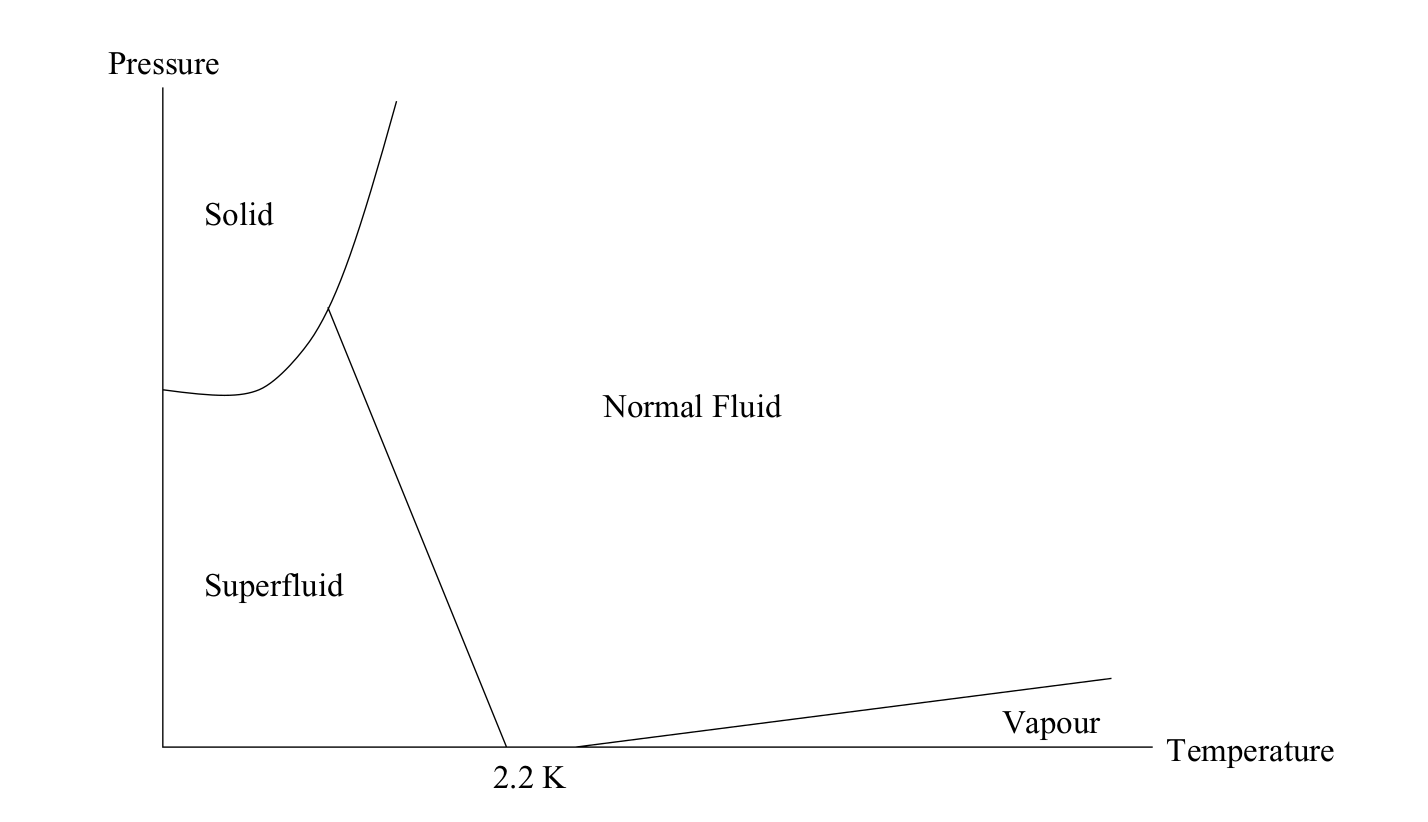
\includegraphics[scale=0.15]{SM/He1.png}
\caption{The phase structure of \ce{^{4}He} at low temperature}
\end{figure}
Helium I is a normal fluid and has a normal gas-liquid critical point. Helium II is a mixture of a normal fluid and a superfluid. 
The superfluid is characterized by the vanishing of its viscosity. Helium I and helium II are separated by a line known as the $\lambda$-transition line.  At $T_{\lambda} = 2.18\mathrm{K}$, $P_{\lambda} = 2.29\mathrm{Pa}$, helium I, helium II, and helium gas coexist. 
The specific heat of liquid helium along the vapour transition line forms a logarithmic discontinuity. The form of this diagram resembles the Greek letter $\lambda$ and is the reason for calling the transition a $\lambda$ transition.
\begin{figure}[!h]
\centering
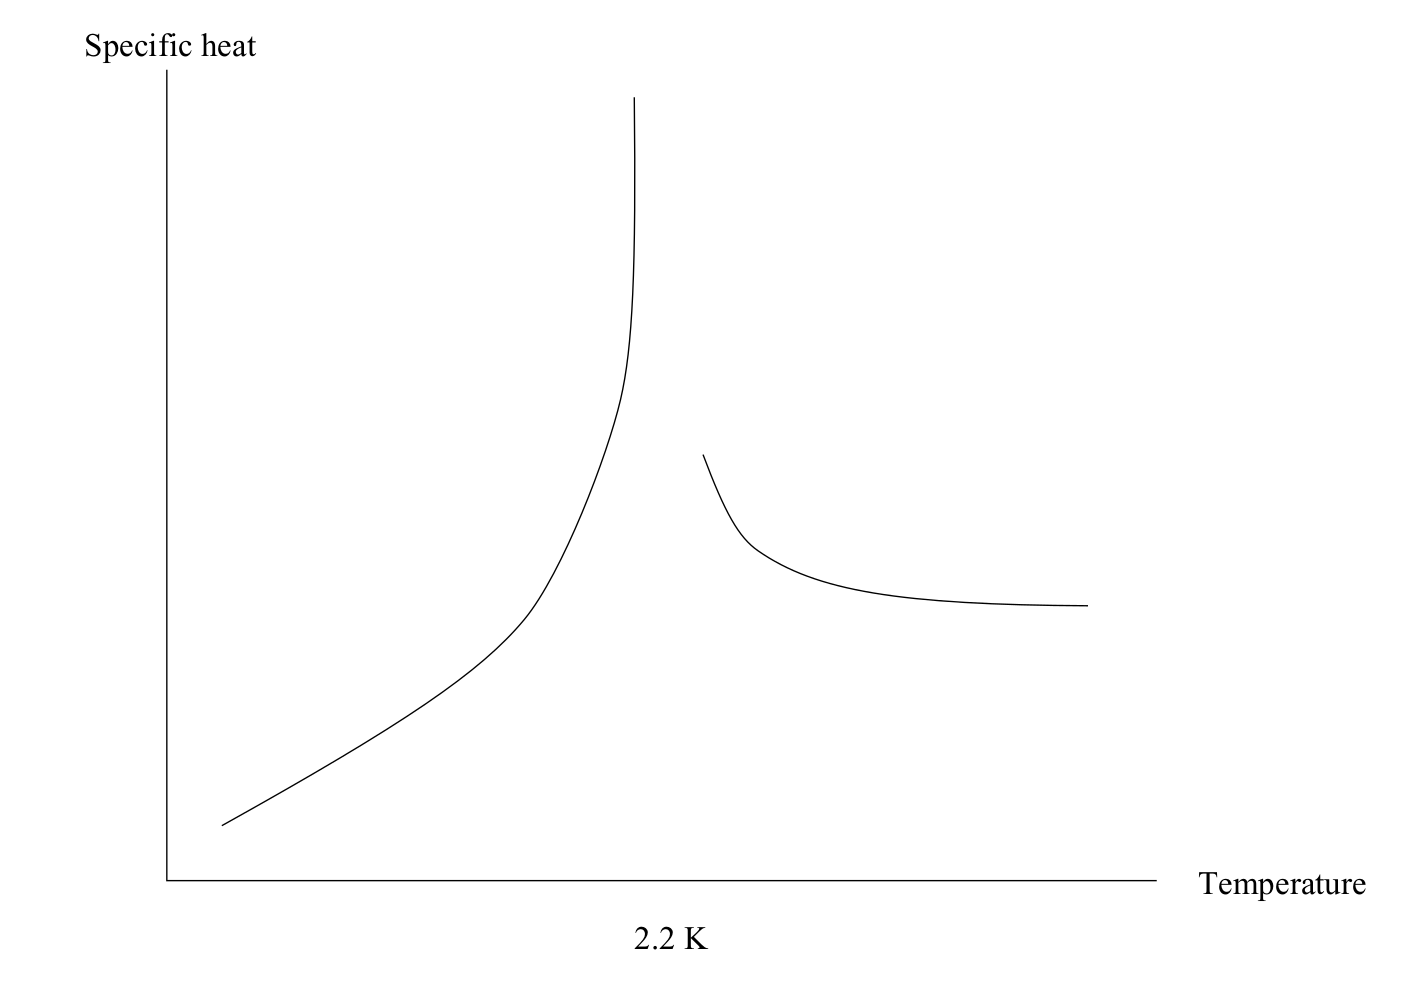
\includegraphics[scale=0.12]{SM/He2.png}
\caption{The specific heat of helium as a function of temperature}
\end{figure}
\\
The excitation spectrum of helium II can be measured experimentally through elastic neutron scattering. It is found to consist of two parts, the phonon region
\[E(\bm{p}) = c|\bm{p}| \quad \mbox{ when } |\bm{p}| \ll |\bm{p}_0|\]
and the roton region
\[E(\bm{p}) = \Delta + \frac{1}{2\mu} |\bm{p} - \bm{p}_0|^2 \quad \mbox{ when } |\bm{p}| \sim |\bm{p}_0|\]
where $c = 226 \mathrm{m/s}$ is the velocity of sound, $\Delta/k_B = 9\mathrm{K}$ are the roton parameters, and $\mu = 0.25m_{He}$. 
There is another velocity parameter known as the critical velocity $v_0$. It is only when helium II moves with velocity greater than $v_0$ that viscous effects arise. At low temperature the roton excitations are damped by the Boltzmann factor $\exp(-\beta \Delta)$.

\subsection{Quantum field theory formulation}
Recall the non-relativistic quantum field theory we develop in quantum mechanics.
The Hamiltonian of a system of \ce{^{4}He} in momentum space is
\[H = \sum_{\bm{k}} \frac{|\bm{k}|^2}{2m} a_{\bm{k}}^{\dagger} a_{\bm{k}} + \frac{1}{2V} \sum_{\bm{k}_1,\bm{k}_2,\bm{q}} \tilde{V}(\bm{q}) a^{\dagger}_{\bm{k}_1 + \bm{q}} a^{\dagger}_{\bm{k}_2-\bm{q}} a_{\bm{k}_1} a_{\bm{k}_2}\]
where
\[a_{\bm{k}} = \frac{1}{\sqrt{V}} \int d\bm{x}\psi(\bm{x}) e^{-i\bm{p}\cdot\bm{x}}\]
and
\[\tilde{V}(\bm{q}) = \int d\bm{x} V(\bm{x}) e^{-i\bm{q}\cdot\bm{x}}\]
Here we adopt box normalization to make momentum of the particle discrete. It is easy to verify that
\[[a_{\bm{p}},a_{\bm{q}}^{\dagger}] = \delta_{\bm{p},\bm{q}} \quad [a_{\bm{p}},a_{\bm{q}}] = 0 \quad [a^{\dagger}_{\bm{p}},a^{\dagger}_{\bm{q}}] = 0\]
The partition canonical partition function is
\[Z = \mathrm{Tr}[e^{-\beta H}]\]
At low temperature, states with low energy value become dominant. These are expected to be states with low values of momentum. 
Let us consider the system close to $T \approx 0$. 
We can then assume that the state of lowest energy corresponds to atoms of low momentum with a sizable fraction of molecules in the zero momenta state, leading to Bose-Einstein condensation. 
Thus if the system has on average $N$ atoms then a significant number $N_0$ of the atoms are in the lowest energy state. More precisely we suppose that the ratio $N_0 / N$ converges to a constant in the limit $N \to \infty$. 
Let us suppose that $|C;N,N_0\rangle$ is a superfluid state with a total of $N$ helium atoms, $N_0$ of which are in the zero momentum plane wave state. 
If $a_0^{\dagger}$ and $a_0$ are creation and destruction operators for a state of zero momentum, we have
\[a_0^{\dagger}a_0 |C;N,N_0\rangle = N_0 |C;N,N_0\rangle\]
and
\[a_0a_0^{\dagger} |C;N,N_0\rangle = (N_0+1) |C;N,N_0\rangle\]
For large $N_0$ we can approximate $N_0 + 1$ by $N_0$ so that on the state $|C;N,N_0\rangle$ we can replace both the operators $a_0^{\dagger}a_0$ and $a_0^{\dagger}a_0$ by a single c-number, $N_0$.

\subsection{The quasi-particle approach}
For $|C;N,N_0\rangle$, the particle number operator $\hat{N}$ can be written as
\[\hat{N} = N_0 + \sum_{\bm{k}\neq 0}a_{\bm{k}}^{\dagger} a_{\bm{k}} \]
Neglecting terms of order $O(N_0^0)$, we have
\[N^2 \approx N_0^2 + 2N_0\sum_{\bm{k}\neq 0}a_{\bm{k}}^{\dagger} a_{\bm{k}} \]
We next examine the interaction part of $H$ when restricted to $|C\rangle$. When all four operators in H I have zero momentum, we have the term
\[H_I^0 = \frac{1}{2V} \tilde{V}(0) a^{\dagger}_{0} a^{\dagger}_{0} a_{0} a_{0} = \frac{1}{2V}\tilde{V}(0)N_0^2 \approx  \frac{1}{2V}\tilde{V}(0) \left[\hat{N}^2-2N_0\sum_{\bm{k}\neq 0}a_{\bm{k}}^{\dagger} a_{\bm{k}} \right]\]
The next term is of order $N_0$ and is the part of $H_I$ containing two operators (carrying zero momentum). There are six ways in which this can happen. If we make an additional assumption that, for $|\bm{k}|$ small, $\tilde{V}(\bm{k}) = \tilde{V}(0)$. 
Since at low temperature we expect only small momenta excitations to be important we replace $\tilde{V}(\bm{k})$ by $\tilde{V}(0)$ in $H_I$. Therefore, on the state , the interacting Hamiltonian, keeping terms of $O(N_0)$ is given by
\[H_I \approx \tilde{V}(0) \left\{ \frac{1}{2V}\left[N^2-2N_0\sum_{\bm{k}\neq 0}a_{\bm{k}}^{\dagger} a_{\bm{k}} \right]  +\frac{N_0}{2V}\sum_{\bm{k}\neq 0} [a^{\dagger}_{\bm{k}} a^{\dagger}_{-\bm{k}} + a_{\bm{k}} a_{-\bm{k}}] +\frac{2N_0}{V} \sum_{\bm{k}\neq 0}a_{\bm{k}}^{\dagger} a_{\bm{k}} \right\} \equiv H_I^B \] 
and the total Hamiltonian can be approximated by the Bogoliubov Hamiltonian $H_B$ given by
\[H^B = \sum_{\bm{k}} \frac{|\bm{k}|^2}{2m} a_{\bm{k}}^{\dagger} a_{\bm{k}} + H_I^B = \sum_{\bm{k}\neq 0} \left(\frac{|\bm{k}|^2}{2m} + \frac{\tilde{V(0)}}{V}N_0 \right)a_{\bm{k}}^{\dagger} a_{\bm{k}}  + \frac{\tilde{V}(0)N_0}{2V} \sum_{\bm{k}\neq 0} [a^{\dagger}_{\bm{k}} a^{\dagger}_{-\bm{k}} + a_{\bm{k}} a_{-\bm{k}}]\]
\\
We turn next to the problem of determining the energy eigenvalues of this Hamiltonian. This we do by using the method of the Bogoliubov–Valatin transform. 
The idea is this: $H_B$ is a quadratic function of the operators $a_{\bm{k}}$ and $a^{\dagger}_{\bm{k}}$. 
By taking appropriate linear combinations of these operators we can form new operators $b_{\bm{k}}$ and $b^{\dagger}_{\bm{k}}$ which "diagonalize" $H^B$, i.e. which lead to
\[H^B = \sum_{\bm{q} \neq 0} \mathcal{E}(\bm{k})b^{\dagger}_{\bm{k}} b_{\bm{k}} \]
The function $\mathcal{E}(\bm{k})$  will then determine the different excitations of the system while $b_{\bm{k}}$ and $b^{\dagger}_{\bm{k}}$ will be destruction and creation operators for these excitations or "quasi-particles", provided they satisfy the commutation rules
\[[b_{\bm{p}},b_{\bm{q}}^{\dagger}] = \delta_{\bm{p},\bm{q}}\]
We write
\[b_{\bm{k}} = \alpha(\bm{k})a_{\bm{k}} - \beta(\bm{k})a^{\dagger}_{-\bm{k}} \quad b^{\dagger}_{\bm{k}} = \alpha(\bm{k})a^{\dagger}_{\bm{k}} - \beta(\bm{k})a_{-\bm{k}} \]
And we have the constraint
\[\alpha(\bm{k})^2 - \beta(\bm{k})^2 = 1\]
Substituting $a$ and $a^{\dagger}$ with $b$ and $b^{\dagger}$ in $H^B$ and comparing it with the $\sum_{\bm{q} \neq 0} \mathcal{E}(\bm{k})b^{\dagger}_{\bm{k}} b_{\bm{k}}$, we can can a set of equations of $\alpha(\bm{k})$ and $\beta(\bm{k})$. Finally, we have
\[\mathcal{E}(\bm{k}) = \sqrt{\frac{\bm{k}^2}{2m} \left(\frac{\bm{k}^2}{2m} + \frac{2N_0\tilde{V}(0)}{V} \right) }\]
The energy $\mathcal{E}(\bm{k})$ is called the quasi-particle energy and the operators $b_{\bm{k}}$ and $b^{\dagger}_{\bm{k}}$ are quasi-particle destruction and creation operators. 
For small values of $\bm{k}$ we have
\[\mathcal{E}(\bm{k}) = \frac{|\bm{p}|}{m} \sqrt{\frac{N_0}{V}\tilde{V}(0)m}\]
Observe that for $\mathcal{E}(\bm{k})$ to be real we must have $\tilde{V}(0) > 0$. This implies there is a repulsive region for $V(x)$ which must dominate the integral $\int dx V(x)$. Observe also that $|\bm{k}|/m = \bm{v}$ is a velocity, and $N_0m/V = \rho$, is the density of the superfluid helium so that the quasi-particle energy can be written as 
\[\mathcal{E}(\bm{p} = m\bm{v}) \approx |\bm{v}|\sqrt{\rho\tilde{V}(0)}\]
\\
We now show that a system with such an energy spectrum represents a superfluid, i.e. a system with no friction.
Friction in a system represents dissipation of energy.
Consider a molecule of mass $M_A$ moving in a medium. If this molecule can change its energy through collisions with the excitations of the medium, then the system has friction. 
We will find that a molecule of mass $M_A$ and velocity $\bm{V}_A$ moving through a system consisting of quasi-particles of energy $\mathcal{E}(\bm{k})$ cannot change its energy by scattering off quasi-particles if $|\bm{V}_A| < |\bm{v}_0|$ where $|\bm{v}_0|$ is a critical velocity determined by $\tilde{V}(0)$ and $\rho$. 
Thus for $|\bm{V}_A| < |\bm{v}_0|$ the system of quasi-particles behaves as a frictionless superfluid.
\\
To see this, let us consider the collision of a molecule of mass $M_A$ and velocity $\bm{V}_A$ with a quasi-particle at rest. If the final momentum of the molecule is $\bm{Q}_A$ and that of the quasi-particle is $\bm{k}$, we have, from momentum conservation,
\[|\bm{Q}_A|^2 = |\bm{P}_A|^2 + |\bm{k}|^2 - 2|\bm{P}_A||\bm{k}|\cos\theta\]
We then have
\[\frac{|\bm{P}_A|^2-|\bm{Q}_A|^2}{2|\bm{P}_A| |\bm{k}|} \leq \frac{|\bm{P}_A|^2-|\bm{Q}_A|^2 + |\bm{k}|^2}{2|\bm{P}_A| |\bm{k}|} = \cos\theta \leq 1\]
Combining this with the energy conservation condition
\[\frac{|\bm{Q}_A|^2}{2M_A} = \frac{|\bm{P}_A|^2}{2M_A} + \mathcal{E}(\bm{p})\]
we end up with
\[\frac{M_A\mathcal{E}(\bm{k})}{|\bm{P}_A| |\bm{k}|} = \frac{1}{m}\sqrt{\frac{\tilde{V}(0)N_0m}{V}} \frac{1}{V_A} \leq 1\]
Thus the process of changing energy for the molecule is not allowed if $V_A \leq v_0 = \frac{1}{m}\sqrt{\frac{\tilde{V}(0)N_0m}{V}} $ and the system of quasi-particles behaves like a superfluid.

\section{Finite temperature perturbation theory}
In this section we develop a perturbative formalism for the computation of the grand canonical partition function. This proceeds in close analogy with the perturbative evaluation of the evolution operator. The grand canonical partition sum 
\[Z_{\Omega} = \mathrm{Tr}e^{-\beta K}\]
where
\[K \equiv K_0 + H_{\mathrm{int}} \equiv H_0 + H_{\mathrm{int}} -\mu N\]
Define
\[U(\beta) \equiv \exp(-\beta K) \quad U_0(\beta) \equiv \exp(-\beta K_0) \quad W(\beta) = U_0^{\dagger}(\beta)U(\beta)\]
Similar to the time-dependent perturbation theory in quantum mechanics, we can get
\[\frac{\partial W}{\partial \beta} = -H_I(\beta)W(\beta)\]
where
\[H_I(\beta) = U_0^{\dagger}(\beta)H_{\mathrm{int}}U_0(\beta)\]
The solution of the equation above can be represented by Dyson series
\[W(\beta) = \sum_{n \geq 0} \frac{(-1)^n}{n!} \int_0^{\beta}d\tau_1 \cdots \int_0^{\beta} d\tau_n T[H_I(\tau_1)\cdots H_I(\tau_n)]\]
Note that $T$ is now the ordering with respect to $\tau$ (or imaginary time). Finally, upon substitution of this last expression into the grand canonical partition sum
\[Z_{\Omega} = \mathrm{Tr} e^{-\beta K_0}W(\beta)\]
we obtain a perturbative expansion of the partition sum in analogy with that of the evolution operator. Before we can apply this formalism to the computation of $Z_{\Omega}$ we need to analyze the finite temperature versions of the time-ordered Green functions and Wick's theorem. The detailed discussion can be found in section 9.8 from \emph{Elements Of Statistical Mechanics (ivo Sachs, Siddhartha Sen, James Sexton)}.

\section{Path integrals}
Similar to the time evolution operator in quantum mechanics, the partition function can be calculated through path integral. We firstly note that
\[e^{-\epsilon(T+V)} = e^{-\frac{\epsilon}{2} V}e^{-\epsilon T} e^{-\frac{\epsilon}{2} V} + O(\epsilon^3)\]
So if we define
\[\epsilon \equiv \frac{\beta}{n}\]
we have
\[\mathrm{Tr}e^{-\beta H} = \mathrm{Tr} \left( e^{-\epsilon H} \right)^n = \mathrm{Tr} \left(e^{-\frac{\epsilon}{2} V}e^{-\epsilon T} e^{-\frac{\epsilon}{2} V}\right)^n + nO(\epsilon^3) = \mathrm{Tr} \left(e^{-\epsilon V}e^{-\epsilon T} \right)^n + O(\epsilon^2)\]
In the limit $n \to \infty$ the error term will go to zero, and we have achieved a splitting of the original exponential operator
\[\mathrm{Tr}e^{-\beta H} = \lim_{n \to \infty} \mathrm{Tr} \left(e^{-\epsilon V}e^{-\epsilon T} \right)^n\]
At this point we are still working with operators, but we can now insert a complete set of states between each term in the product, and convert the problem to one with just commuting numbers. For simplicity, we assume the system has only one pair of canonical variables.
\begin{eqnarray}
&\phantom{=}& \mathrm{Tr}e^{-\beta H} \nonumber \\
&=& \lim_{n \to \infty} \int [dpdq]^n  \mathrm{Tr} [ e^{-\epsilon V}|q_0\rangle \langle q_0 | e^{-\epsilon T} |p_0 \rangle\langle p_0| e^{-\epsilon V} \cdots e^{-\epsilon V} |q_{n-1}\rangle\langle q_{n-1}| e^{-\epsilon T} |p_{n-1}\rangle\langle p_{n-1} | ] \nonumber \\
&=& \lim_{n \to \infty} \int [\frac{dpdq}{2\pi}]^n e^{\sum_{i=0}^{n-1}ip_i(x_{i+1}-x_i) - \epsilon H(q_i,p_i)} \nonumber
\end{eqnarray}
where $q_{n} = q_0$. 
Generally, we have $T(p) = \frac{p^2}{2m}$. The $p_k$ integral is just a Gaussian integral. The path integral can then be simplified to
\[\mathrm{Tr}e^{-\beta H} = \lim_{n \to \infty} \left( \frac{m}{2\pi \epsilon} \right)^{\frac{n}{2}} \int [dq]^n e^{\epsilon \sum_{i=0}^{n-1}  -\frac{m}{2\epsilon^2}(q_{i+1}-q_i)^2 -  V(q_i)} \]
Similar to path integral formulation in quantum mechanics, the equation above can be written formally as
\[\mathrm{Tr}e^{-\beta H} = \int \mathcal{D}q(\tau) e^{S_E(q(\tau))}\]
with constraint $q(0) = q(\tau)$
where
\[S_E[q(\tau)] = \int_0^{\beta} -\frac{m}{2}\dot{q}^2 - V(q)\]
In quantum mechanics, we have
\[\langle b | e^{-iHT} | a \rangle = \int \mathcal{D}q(t) e^{iS(q(t))}\]
with constraint $q(0) = a$ ans $q(\tau) = b$
where
\[S[q(t)] = \int_0^{T} \frac{m}{2}\dot{q}^2 - V(q)\]
Actually, path integral of quantum mechanics can be obtained directly if we replace $\beta$ with $iT$ and change the integral variable from $\tau$ to $t$ by $\tau = it$ in the path integral  of statistical mechanics.
\\ \\
The path integral formulation can be generalize to the case of quantum field directly. For the system of bosons, we have
\[\mathrm{Tr}e^{-\beta H} = \int \mathcal{D}\psi \mathcal{D}\psi^{\dagger} e^{S_E}\]
with constraint $\psi(\bm{x},0) = \psi(\bm{x},\beta)$
where
\begin{eqnarray}
S_E &=& \int_0^{\beta}d\tau \left[ \int d^3x \psi^{\dagger}(\bm{x},\tau) \left( -\frac{\partial}{\partial \tau} + \frac{\nabla^2}{2m} \right) \psi(\bm{x},\tau) \right. \nonumber \\
&-& \left. \frac{1}{2}\int d^3x d^3y\psi^{\dagger}(\bm{x},\tau)\psi^{\dagger}(\bm{y},\tau)V(\bm{x}-\bm{y})\psi(\bm{x},\tau)\psi(\bm{y},\tau) \right] \nonumber
\end{eqnarray}
As for Fermions, we have
\[\mathrm{Tr}e^{-\beta H} = \int \mathcal{D}\psi \mathcal{D}\psi^{\dagger} e^{S_E}\]
with constraint $\psi(\bm{x},0) = -\psi(\bm{x},\beta)$. 
And the value of $\psi(\bm{x},t)$ is Grassman number rather than $c$ number, which has been discussed in the path integral formulation of Dirac field.

\chapter{Phase Transitions and the Renormalization Group}
\section{Basic problem}
A given equilibrium state of a macroscopic system can be described by an order parameter field. For a ferromagnet the order parameter field is the magnetization density. 
The order parameter field can be regarded as a mapping from the system (with coordinate $\bm{x}$) to an order parameter space. In a model where the magnetization density is given by a scalar function $M_z(\bm{x})$ this is the space of real numbers. In general the order parameter space can be more complicated and the order parameter field need not be a scalar function.
A phase transition corresponds to the order parameter field
changing qualitatively together with the emergence of singular behaviour in the system.
\\ \\
For instance the order parameter field in the case of a ferromagnet is non-zero in the ferromagnetic phase, is zero in the paramagnetic phase, and the susceptibility of the system diverges at the phase transition temperature. 
Determining a suitable order parameter field to characterize a phase is part of the task of a theory of phase transitions. If the order parameter field changes continuously from one phase to another, as in the case of a ferromagnet, the transition is said to be a continuous or second-order phase transition. If it is discontinuous the transition is said to be first order. 
An example of a first order transition is when a solid melts
to a liquid. The density of the system, which can be taken as the order parameter, changes discontinuously. A phase transition is a striking example of an emergent phenomenon. Starting off with only short-range interactions between its microscopic magnetic moments, the system realizes long-range correlations below $T_c$.
\\ \\
We start with a model for a ferromagnet. We regard a ferromagnetic solid as being made out of a finite number of elementary magnets placed at locations throughout the solid.
We simplify our model by assuming that each of these elementary magnets m can either point up $m = 1$ or down $m = -1$. Finally each elementary magnet interacts only with its nearest neighbour. A Hamiltonian for this model could be
\[H = -g\sum_{n,i}m_im_{i+n} - B\sum_i m_i\]
where the first sum is over $i$ as well as the nearest neighbours of $i$. Note $H$ decreases if $m_i$, $m_{i+n}$ have the same sign for $g > 0$. There are altogether a large but finite number of magnets in a ferromagnet. Then we can prove that in the model of a ferromagnet proposed the susceptibility cannot diverge. 
\\
Whereas, the theorem fails if we allow the number of elementary magnets to tend to infinity. This is because an infinite sum of analytic functions need not be analytic. 
In order to analyze this possibility we will need to consider the statistical mechanics partition function in the limit in which the number of configurations is infinite. It is only in this limit that the phase transitions might be understood from this point of view.
\\ \\
Another approach to the problem is to suppose that the external magnetic field $B$ is changed to $B + \delta B(\bm{x})$, i.e. the change $\delta B$ is position dependent. We expect that a change at $\bm{x}$, $\delta B(\bm{x})$, will produce a change in the magnetization $\delta M$ not just at the point $\bm{x}$ but at other points as well. Indeed we might expect
\[\delta M(\bm{y}) \propto C_T(|\bm{x}-\bm{y}|)\delta B(\bm{x})\]
where $C_T$ is a "correlation function" which determines the effect at $\bm{x}$ on the magnetization due to a change in the external field $\delta B$ at $\bm{x}$. The total change
is then expected to be
\[\delta M(\bm{y}) = \int d^3x C_T(|\bm{x}-\bm{y}|)\delta B(\bm{x})\]
We have assumed that the correlation function depends only on temperature and on the distance between the points $\bm{x}$ and $\bm{y}$.
Let us now suppose that $\delta B$ is independent of $\bm{x}$ and let us set $\bm{y} = 0$. Then we have
\[\chi(0) = \frac{\delta M(0)}{\delta B} = \int d^3x C_T(|\bm{x}|)\]
If we suppose
\[C_T(|\bm{x}|) = \begin{cases} \alpha \quad |\bm{x}| \leq a(T) \\ 0 \quad |\bm{x}| > a(T) \end{cases}\]
that is, a disturbance only propagates a distance $a(T)$, then
\[\chi(0) = \frac{4\pi \alpha}{3} a^3(T)\]
Thus $\chi(0)$ will diverge if $a(T)$ diverges, that is, if correlations in the system become infinite. From this point of view the divergence in this susceptibility is due to the fact that near a phase transition disturbances propagate over large distances, $a(T) \to \infty$. 

\section{Landau theory of phase transitions}
Recall that for any change of a system in which the temperature is kept fixed and no work is done by the system, the change of free energy, $\Delta F$, is always negative so that a state of equilibrium must be a minimum of $F$. Landau utilized this property of the free energy in his theory of phase transitions.
\\
Let us examine this approach for the case of a ferromagnet. The basic idea is to make a model for the free energy $F$ near the Curie temperature $T_c$ when the system is still a ferromagnet. We know that for $T < T_c$ long-range correlations are present, that is, the spin at lattice site $\bm{x}$ must point in the same direction as that at site $\bm{y}$ even when $\bm{x}$ and $\bm{y}$ are not adjacent. Otherwise the observed macroscopic magnetic properties of the system would not exist.
\\
The basic assumption underlying Landau's theory is that, near the critical temperature $T_c$, the properties of a ferromagnet can be described in terms of a magnetization density function $M(\bm{x})$. 
The function $M(\bm{x})$ can be defined by considering a volume element $\Delta V$, large compared to the lattice cell volume, but small compared to the volume of correlated spins centred around the point $\bm{x}$. 
The magnetization of the volume element $\Delta V$ is defined to be $M(\bm{x}) \Delta V$. For this definition of $M(\bm{x})$ to be useful it is important that $M(\bm{x})$ should not be a rapidly varying function of position. Near the Curie temperature $T_c$ we also expect $M(\bm{x})$ to be small in amplitude. 
Since we are implicitly assuming in this approach that a spin-spin type of interaction is responsible for the phenomenon of ferromagnetism it seems reasonable to expect the free energy density to be a function of $M(\bm{x})\cdot M(\bm{x})$. On the basis of arguments of this kind Landau proposed to introduce a functional $F_L[T,\bm{B},\bm{M}]$ of the magnetization density $\bm{M}(\bm{x})$, temperature $T$, and external magnetic field $\bm{B}(\bm{x})$ of the form
\[F_L[T,\bm{B},\bm{M}] = F_L(T,\bm{B},0) + \int d^3x \left[ a(T)|M|^2 + b(T)|M|^4 + \cdots + c(T)\sum_{ij} (\nabla_jM_i)^2 + \cdots - \bm{B}\cdot\bm{M} \right]\]
The free energy $F_L(T,\bm{B})$ is then obtained by minimizing $F_L[T,\bm{B},\bm{M}]$ with respect to $\bm{M}$. Note that the temperature dependent coefficients $a(T), b(T), c(T) \cdots$ are assumed to be smooth functions of temperature. We will simplify the model function by assuming  acts along the $z$-direction and that $\bm{M}(x)$ only has components in the $z$-direction. Then we have
\[F_L[T,B_z,M_z] = F_L(T,B_z,0) + \int d^3x \left[ a(T)M_z^2 + b(T)M_z^4 + \cdots + c(T)|\bm{\nabla}M_z|^2 + \cdots - B_z M_z \right]\]
The expression for the Landau free energy $F_L$ is expected to be useful when $T$ is close to the Curie temperature $T_c$ . In this region $M_z(\bm{x})$ is expected to be small and we also expect $|\bm{\nabla}M_z|^2$ to be small. 
Because of these reasons we will from now on ignore the effect of the higher powers of $M_z$ and higher gradient terms. 
To determine the equilibrium configuration of the magnetization we have to minimize the free energy with respect to $M_z(\bm{x})$. Using
\[\delta F_L = \int d^3x [2a(T)M_z + 4b(T)M_z^3 - 2c(T)\nabla^2 M_z - B_z]\delta M_z\]
we see that vanishing of $\delta F$ for arbitrary $\delta M_z$ requires
\[2a(T)M_z(\bm{x}) + 4b(T)M_z^3(\bm{x}) - 2c(T)\nabla^2M_z(\bm{x}) = B_z(\bm{x})\]
Suppose now that $B_z(\bm{x})$ does not depend on $\bm{x}$ and let us see if a solution for $M_z(\bm{x})$ independent of $\bm{x}$ is possible. Such an $\bm{x}$ independent solution must satisfy
\[[2a(T)M_z + 4b(T)M_z^3] = B_z\]
Now we ask if it is possible to construct a solution with the property that $M_z \neq 0$ when $B_z = 0$ and $T < T_c$.
\\ \\
As we have stressed this model is constructed to represent a ferromagnet near its Curie temperature. We also assume that the coefficient functions are all smooth functions of temperature. 
We thus expect the $M_z^4$ term to be small compared to the $M_z^2$ term. It is then reasonable to replace $b(T)$ by $b(T_c) = b_0$, a constant and set $a(T) = a_0(T-T_c)$. If we assume $a_0 > 0$ and $b_0 > 0$, then when $T > T_c$, the solution is
\[M_z = 0\]
When $T < T_c$, the solution is
\[M_z = 0 \mbox{ or } \pm \sqrt{\frac{a_0(T_c-T)}{2b_0}}\]
Note that
\[F(M_z = 0) > F(M_z = \pm \sqrt{\frac{a_0(T_c-T)}{2b_0}})\]
we must have $M_z = \sqrt{a_0(T_c-T)/b_0}$ when $T < T_c$.
\begin{figure}[!h]
\centering
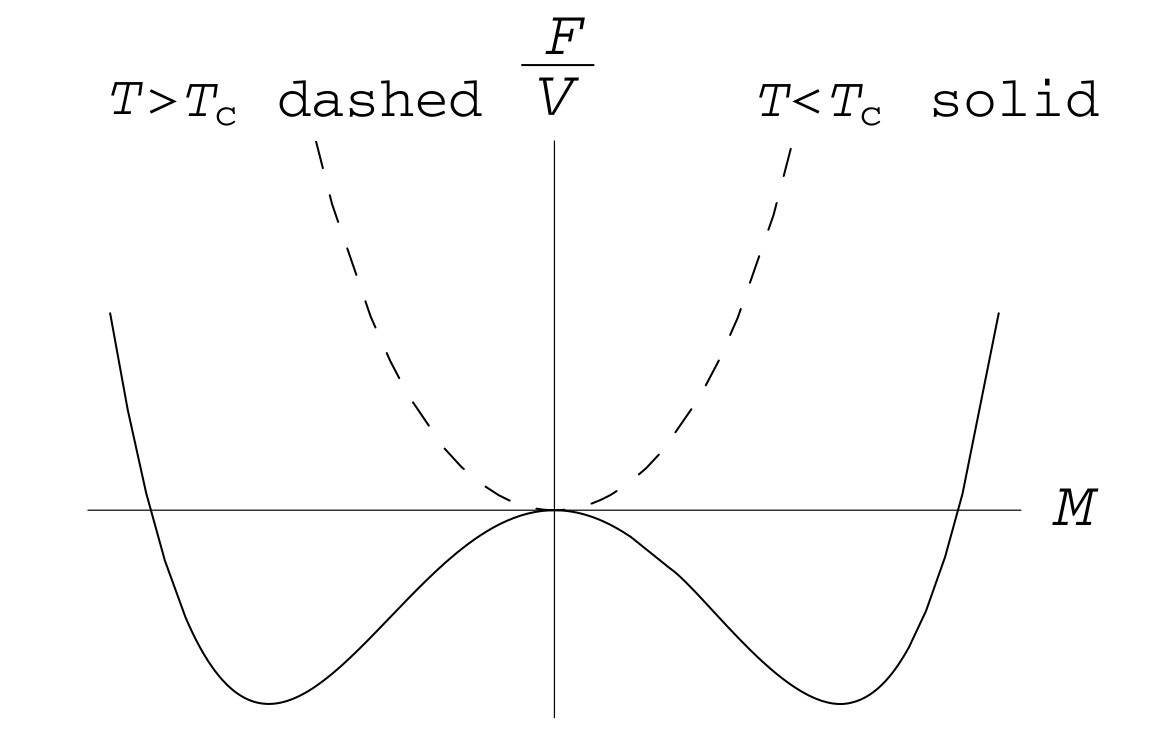
\includegraphics[scale=0.2]{SM/landau.png}
\caption{Landau free energy}
\end{figure}
\\
Furthermore, for $T = T_c$,
\[M_z^3 = \frac{B_z}{4b_0}\]
Finally we note that if $B_z$ is changed to $B_z + \delta B_z$, the corresponding equilibrium distribution $M_z$ can be written as $M_z + \delta M_z$. We thus get
\[2a_0(T-T_c)\delta M_z + 12b_0M_z^2\delta M_z = \delta B_z\]
Setting $B_z = 0$, we find
\[\chi = \left. \frac{\delta M_z}{\delta B_z} \right|_{B_z = 0} = \begin{cases} \frac{1}{2a_0(T-T_c)} \quad T>T_c \\ \frac{1}{4a_0(T_c-T)} \quad T<T_c \end{cases} \]
Landau's theory qualitatively reproduces the expected singular behaviour.
\\ \\
It is also possible to get a rather precise statement regarding long-range correlations within the framework of Landau's theory. Recall that
\[\delta M(\bm{y}) = \int d^3x C_T(|\bm{x}-\bm{y}|)\delta B(\bm{x})\]
From the equations which describe the equilibrium magnetization density we have with $c(T) = c_0$,
\[2a(T)M_z(\bm{x}) + 4b_0M_z^3(\bm{x})- 2c_0\nabla^2M_z(\bm{x}) = B_z(\bm{x})\]
So, we can get
\[[2a_0(T-T_c) + 12b_0M_z^2 - 2c_0\nabla^2] \delta M_z(\bm{x}) = \delta B_z(\bm{x})\]
From these equations it follows that
\[[2a_0(T-T_c) + 12b_0M_z^2 - 2c_0\nabla^2]C_T(|\bm{x} - \bm{y}|) = \delta(\bm{x} - \bm{y}) \]
Setting $B_z = 0$ and rescaling the coordinates as $(\bm{u},\bm{v}) = 2c_0(\bm{x},\bm{y})$ we get
\[[2\bar{a}_0(T-T_c) - \nabla^2] C_T(|\bm{u} - \bm{v}|) = \delta(\bm{u} - \bm{v})\]
where $\bar{a}_0 = a_0/(2c_0)^3$.
This result is valid in the region $T > T_c$ . For $T < T_c$ we get
\[[4\bar{a}_0(T_c-T) - \nabla^2] C_T(|\bm{u} - \bm{v}|) = \delta(\bm{u} - \bm{v})\]
The solution is
\[C_T(|\bm{x} - \bm{y}|) = \frac{1}{4\pi} \frac{e^{-\frac{|\bm{x} - \bm{y}|}{\xi}}}{|\bm{x} - \bm{y}|}\]
where $\xi^2 = c_0/a(T)$ for $T > T_c$ and $\xi^2 = -c_0/2a(T)$ for $T < T_c$.
We notice that $\xi \to \infty$ as $T \to T_c$. Thus Landau's theory is in qualitative agreement with the intuitive idea that long-range correlations are generated in a ferromagnet as $T \to T_c$.
\\
Another point to note is that if $\delta B_z$ were $\bm{x}$ independent, then as we saw before
\[\chi(0) = \frac{\delta M(0)}{\delta B} = \int d^3x C_T(|\bm{x}|) \sim \chi^2 \to \infty \quad \mbox{ as } T \to T_c\]
\\ \\
Let us summarize the results obtained from Landau's approach. The approach focused on long-range correlations and suggested that the singular behaviour of the susceptibility was due to such correlations when $T \to T_c$. 
The approach also predicts that the relation between different macroscopic parameters involves power laws,
\[M_z \sim (T_c - T)^{\beta} \quad T \to T_c\]
\[M_z \sim B_z^{1/\delta} \quad T = T_c\]
\[\chi \sim \frac{1}{(T_c-T)^{\gamma}} \quad T \to T_c\]
with $\beta = \frac{1}{2}$, $\gamma = 1$, and $\delta = 3$. The parameters $\beta$, $\delta$ and $\gamma$ are called critical exponents and are measured experimentally. 
The experimental values for these parameters
$\beta \approx 1.33$, $\delta \approx 4.5$, and $\gamma \approx 1.2$ are found for different ferromagnet with different lattice structures and widely differing values for the Curie temperature $T_c$. 
These parameters thus are a universal property of the ferromagnetic phase transition. This is also a feature of Landau's theory. Thus Landau's theory is in qualitative
agreement with experiment.

\section{Renormalization group}
\subsection{Introduction}
Although Landau's theory is in good qualitative agreement with experiment there is room for improvement on the quantitative level concerning the critical exponents.
Instead of considering a model for the free energy we now consider the partition function directly. 
\\
Let us consider a one-dimensional ferromagnetic system described in terms of an Ising model.
\[Z = \mathrm{Tr}e^{-\beta H}\]
with
\[H = -J\sum_{i=1}^N S_i S_{i+1} - H\sum_{i=1}^N S_i\]
where $S_i = \pm 1$ denotes the (uniaxial) magnetization or spin of site $i$ (periodic boundary conditions, $S_{N+1} = S_1$, imposed), and $H$ represents an external field. We have
\[e^{-\beta H} = e^{\sum_{1}^N KS_iS_{i+1} + hS_i} = \prod_{i=1}^N T(S_i,S_{i+1})\]
where $K = \beta J > 0$ and $h = \beta H$, and the weight is defined through the relation $T(S,S') = \exp[KSS' + \frac{h}{2}(S+S')]$. So,
\[Z = \sum_{\{S_i\}} e^{-\beta H} = \mathrm{Tr}T^N\]
and
\[T = \begin{pmatrix}
e^{K+h} & e^{-K} \\ e^{-K} & e^{K-h}
\end{pmatrix}\]
Following the program outlined by Kadanoff's seminal work on the foundations of the RG, we will follow a strategy whereby this renormalization step may be effected by subdividing the spin chain into regular clusters of b neighbouring spins. We may then proceed to sum over the $2b$ sub-configurations of each cluster, thereby generating an effective functional describing the inter-cluster energy balance. 
While it is clear that this energy functional exists, a far less obvious question to ask is whether it will again have the form of an effective Ising spin system. Remarkably, the answer is affirmative: the Ising model is said to be "renormalizable." 
The structural reproduction of the model implies that we can think of each cluster as some kind of meta-Ising spin, or block spin. More importantly, it guarantees that the renormalization step qualifies for iteration: in a second RG step, $b$ block spins are grouped to form a new cluster (now comprising $b^2$ of the microscopic spins) which are then traced out, etc. We have
\[Z_{N}(K,h) = \mathrm{Tr} T^N = \mathrm{Tr} (T^b)^{N/b} =\mathrm{Tr} (T')^{N/b} = Z_{N/b}(K',b')\]
Define $u \equiv e^{-K}$ and $v \equiv e^{-h}$, we can work out
\[u' = \frac{\sqrt{v+v^{-1}}}{(u^4 + u^{-4} + v^2 + v^{-2})^{1/4}} \quad v' = \frac{\sqrt{u^4 + v^2}}{\sqrt{u^4 + v^{-2}}}\]
The possibility of representing the new transfer matrix in the same algebraic structure as the old one implies that the transformed model again describes an Ising spin system. However, the Hamiltonian $\beta H$ of the new block spin system is defined at a different temperature, magnetic field and exchange constant and describes fluctuations on length scales that are twice as large as in the original system.
In particular, the short-distance cut-off has been doubled.
\\ \\
To make further progress, one may focus on the two relevant parameters $u'$ and $v'$ and observe that the result of the block spin transformation can be represented as a discrete map
\[\begin{pmatrix} u' \\ v' \end{pmatrix} = \begin{pmatrix}
f_1(u,v) \\ f_2(u,v)
\end{pmatrix} \]
In one-dimensional Ising model, the map $f$ possesses two
disjoint sets of fixed points $(u^*,v^*) = (0,1)$ and $(u^*,v^*) = (1,v)$.
\\
The set of fixed points represents the most important structural characteristic of an RG analysis. They organize the space of "flowing" coupling constants into sectors of qualitatively different behaviour. 
In particular, one may note that, at a fixed point, all characteristics of the model, including its correlation length $\xi$, remain invariant. 
On the other hand, we noticed above that an RG step is tantamount to doubling the fundamental length scale of the system. Consistency requires that either $\xi = 0$ or $\xi = \infty$. 
In the present case, the line of fixed points is identified with $u = \exp[-\beta J] = 1$, i.e. $\beta = 0$. 
This is the limit of infinitely large temperatures, at which we expect the model to be in a state of maximal thermal disorder, that is $\xi = 0$. 
Besides the high-temperature fixed line, there is a zero-temperature fixed point $(u, v) = (\exp[−\beta J], \exp[−\beta h]) = (0, 1)$ implying $T \to 0$ and $h \to 0$. Upon approaching zero temperature, the system is expected to order and to build up long-range correlations, $\xi \to \infty$. And we can say critical point corresponds to a fixed point of RG group with infinity correlation length.
\\
Notice, however, an important difference between the high- and the low-temperature set of fixed points: while the former is an attractive fixed point in the sense that the RG trajectories approach it asymptotically, the latter is a repulsive fixed point. No matter how low the temperature at which we start, the RG flow will drive us into a regime of effectively higher temperature or lower ordering. 
(Of course, the physical temperature does not change under renormalization. All we are saying is that the block spin model behaves as an Ising model at a higher temperature than the original system.)
\\
A detailed discussion of one-dimensional Ising model can be found in section 8.1 from \emph{Condensed Matter Field Theory (Alexander Altland \& Ben Simons)}. A discussion of a model with continuous configurations can be found in section 8.2 of the same book. The model implements RG by integrating out fields with high frequency modes. The same method can also be used in relativistic quantum  field theory. A detail discussion can be found in section 12.1 form \emph{An introduction to quantum field theory (M.E.Peskin \& D.V.Schroeder)}

\subsection{Gell-Mann-Low equations}
There are a number of methodologically different procedures whereby the set of flow equations can be obtained from the microscopic theory. Here, we formulate this step in a language adjusted to applications in statistical field theory as opposed to particle physics. While there is considerable freedom in the actual implementation of the RG procedure, all methods share the feature that they proceed in a sequence of three more or less canonical steps.
\subsubsection{Subdivision of the field manifold}
In the first step, one may decompose the integration manifold $\{\phi\}$ into a sector to be integrated out, $\{\phi_f\}$, and a complementary set, $\{\phi_s\}$.
\begin{itemize}
\item We may proceed according to a generalized block spin scheme and integrate over all degrees of freedom located within a certain structural unit in the base manifold $\{\bm{x}\}$.(This scheme is adjusted to lattice problems where $\{\bm{x}\} = \{\bm{x}_i\}$ is a discrete set of points.)
\item We could decide to integrate over a certain sector in momentum space. When this sector is defined to be a shell $\Lambda /b < |\bm{p}| < \Lambda$, one speaks of a momentum shell integration. Naturally, within this scheme, the theory will be explicitly cutoff-dependent at intermediate stages.
\item Alternatively, we may decide to integrate over all high-lying degrees of freedom $\lambda^{-1} \leq |\bm{p}|$.
In this case, we will of course encounter divergent integrals. An elegant way to handle these divergences is to apply dimensional regularization. Within this approach one formally generalizes from integer dimensions $d$ to fractional values $d \pm \epsilon$. 
One motivation for doing so is that the formal extension of the characteristic integrals appearing during the RG step to non-integer dimensions are finite. As long as one stays clear of the dangerous values $d = \mbox{ integer}$ one can then safely monitor the dependence of the integrals on the IR cutoff $\lambda^{-1}$.
\end{itemize}

\subsubsection{RG step}
The second part of the program is to actually integrate over short range fluctuations. This step usually involves approximations. 
In most cases, one will proceed by a so-called loop expansion, i.e. one organizes the integration over the fast field $\phi_f$ according to the number of independent momentum integrals -loops - that occur after the appropriate contractions.
\\
Following the procedure, an expansion over the fast degrees of freedom gives an action in which coupling constants of the remaining slow fields are altered. 
Notice that the integration over fast field fluctuations may  lead to the generation of "new" operators, i.e. operators that have not been present in the bare action. In such cases one has to investigate whether the newly generated operators are "relevant" in their scaling behaviour. 
If so, the appropriate way to proceed is to include these operators in the action from the very beginning (with an a priori undetermined coupling constant). One then verifies whether the augmented action represents a complete system, i.e. one that does not lead to the generation of operators beyond those that are already present. If necessary, one has to repeat this step until a closed system is obtained.

\subsubsection{Rescaling}
One next rescales frequency/momentum so that the rescaled field amplitude $\phi'$ fluctuates on the same scales as the original field $\phi$, i.e. one sets
\[q \to bq \quad \omega \to b^z \omega\]
Here, the frequency renormalization exponent or dynamical exponent $z$ depend on the effective dispersion relating
frequency and momentum. 
We finally note that the field $\phi$, as an integration variable, may be rescaled arbitrarily. Using this freedom, we select a term in the action which we believe governs the behaviour of the "free" theory - in a theory with elastic coupling this might be the leading-order gradient operator $\int d^d r (\nabla \phi)^2$ - and require that it be strictly invariant under the RG step. 
To this end we designate a dimension $L^{d_{\phi}}$ for the field, chosen so as to compensate for the factor $b^x$ arising after the renormalization of the operator. The rescaling $\phi \to b^{d_{\phi}}$ is known as field renormalization. It renders the "leading" operator in the action scale invariant.
\\ \\
As a result of all these manipulations, we obtain a renormalized action
\[S[\phi] = \sum_a g'_a \mathcal{O}_a[\phi]\]
which is entirely described by the set of changed coupling constants, i.e. the effect of the RG step is fully encapsulated in the mapping
\[\bm{g}' = \tilde{R}(\bm{g})\]
relating the old value of the vector of coupling constants to the renormalized one. 
By letting the control parameter, $l \equiv \ln b$, of the RG step assume infinitesimal values, one can make the difference between bare and renormalized coupling constants
arbitrarily small. 
It is then natural to express the difference in the form of a generalized $\beta$-function or Gell-Mann-Low equation
\[\frac{d\bm{g}}{dl} = R(\bm{g})\]
where the right-hand side is defined through the relation
\[R(\bm{g}) = \lim_{l \to 0} l^{-1} (\tilde{R}(\bm{g}) - \bm{g})\]
\\
Actually Gell-Mann-Low equation here is the same equation as the one in relativistic quantum field theory which describe the flow of coupling coefficient with the energy scale of the experiment. Suppose the cutoff of the theory is $\Lambda_0$, the energy scale of the experiment is $\mu$, and $\lambda_i$ is the coupling coefficient in the theory with dimension $[\mbox{energy}] ^{d_{i}}$. If the dimension of the physical quantity we want to measure is $d_Q$, then generally, we have
\[\frac{Q}{\Lambda_0^{d_O}} = F(\frac{\mu}{\Lambda_0},\frac{\lambda_i}{\Lambda_0^{d_i}})\]
Then, we can integrate out the high frequency mode between $\mu$ and $\Gamma_0$ of the theory and rescale the energy and momentum to get the new coupling coefficient $\lambda(b)$, where $b = \Lambda_0 / \mu$. So, in the new effective theory, we have
\[\frac{Q}{\mu^{d_O}} = F(1,\frac{\lambda_i(\Lambda_0 / \mu)}{\mu^{d_i}})\]
The flow of coupling coefficient given by
\[\frac{d\lambda}{d\ln \mu} = - \frac{d\lambda}{d\ln b}\]

\subsection{Analysis of the Gell-Mann-Low equation}
The prime structural characteristic of the Gell-Mann-Low equations is the set of fixed points, i.e. the submanifold $\{\bm{g}^*\}$ of points in coupling constant space which are stationary under the flow. 
Once the coupling constants are fine-tuned to a fixed point, the system no longer changes under subsequent RG transformations. In particular it remains invariant under the change of space/time scale associated with the transformation.
Alluding to the fact that they look the same no matter how large a magnifying glass is used, systems with this property are referred to as self-similar.
\\
Now, to each system, one can attribute at least one intrinsic length scale, namely the length $\xi$ determining the exponential decay of field correlations. 
However, the existence of a finite, and pre-determined, intrinsic length scale clearly does not go together with invariance under scale transformations. We thus conclude that, at a fixed point, either $\xi = 0$ (not so interesting), or $\xi = \infty$. 
However, a diverging correlation length $\xi \to \infty$ is a hallmark of a second-order phase transition. We thus tentatively identify fixed points of the RG flow as candidates for "transition points" of the physical system.
\\
This being so, it is natural to pay special attention to
the behaviour of the flow in the immediate vicinity of the fixed-point manifolds. If the set of coupling constants, $g$, is only close enough to a fixed point, $g^*$, it will be sufficient to consider the linearized mapping
\[R(\bm{g}) \equiv R[g^*+(g-g^*)] \approx W(g-g^*) \quad W_{ab} = \left. \frac{\partial R_a}{\partial g_b} \right|_{g=g^*}\]
To explore the properties of flow, let us assume that we had managed to diagonalize the matrix $W$ . Denoting the eigenvalues by $\lambda_{\alpha}$, and the left-eigenvectors by $\phi_{\alpha}$, we have
\[\phi_{\alpha}^T W = \phi_{\alpha}^T\lambda_{\alpha}\]
let $v_{\alpha}$ be the $\alpha$th component of the vector $\bm{g} - \bm{g}^*$ when represented in the basis $\{\phi_{\alpha}\}$:
\[v_{\alpha} = \phi_{\alpha}^T (\bm{g}-\bm{g}_{*})\]
We can easily derive that
\[\frac{dv_{\alpha}}{dl} = \lambda_{\alpha}v_{\alpha}\]
Under renormalization, the coefficients $v_{\alpha}$ change by a mere scaling factor $\lambda_{\alpha}$, wherefore they are called scaling fields.
\[v_{\alpha}(l) \sim \exp(l\lambda_{\alpha})\]
This result suggests a discrimination between at least three different types of scaling fields
\begin{itemize}
\item For $\lambda_{\alpha} > 0$ the flow is directed away from the critical point. The associated scaling field
is said to be relevant (in the sense that it forcefully drives the system away from the critical region).
\item In the complementary case, $\lambda_{\alpha} < 0$, the flow is attracted by the fixed point. Scaling fields
with this property are said to be irrelevant.
\item Finally, scaling fields which are invariant under the flow, $\lambda_{\alpha} = 0$ , are termed marginal.
\end{itemize}
The distinction of relevant/irrelevant/marginal scaling fields in turn implies a classification of different types of fixed points:
\begin{itemize}
\item Firstly, there are stable fixed points, i.e. fixed points whose scaling fields are all irrelevant or, at worst, marginal. 
These points define what we might call "stable phases of
matter": when you release a system somewhere in the parameter space surrounding any of these attractors, it will scale towards the fixed point and eventually sit there. Or,
expressed in more physical terms, looking at the problem at larger and larger scales will make it more and more resemble the infinitely correlated self-similar fixed-point configuration. (Recall the example of the high-temperature fixed line of the one-dimensional Ising
model encountered earlier.) 
By construction, the fixed point is impervious to moderate
variations in the microscopic morphology of the system, i.e. it genuinely represents what one might call a "state of matter."
\item Complementary to stable fixed points, there are unstable fixed points. Here, all scaling fields are relevant (the $T = 0$ fixed point of the 1-D Ising model). These fixed points represent the concept of a Platonic ideal: you can never get there and, even if you managed to approach it closely, the harsh conditions of reality will make you flow away from it.
Although unstable fixed points do not correspond to realizable forms of matter, they are of importance inasmuch as they "orient" the global RG flow of the system.
\item Finally, there is the generic class of fixed points with both relevant and irrelevant scaling fields. These points are of particular interest inasmuch as they can be associated with phase transitions. 
To understand this point, we first note that the $r$ eigenvectors $\phi_{\alpha}$ associated with irrelevant scaling fields span the tangent space of an $r$-dimensional
manifold known as the critical surface. 
This critical manifold forms the basin of attraction of the fixed point, i.e. whenever a set of physical coupling constants $g$ is fine-tuned so that $g \in S$, the
expansion in terms of scaling fields contains only irrelevant contributions and the system will feel attracted to the fixed point as if it were a stable one.
\\
However, the smallest deviation from the critical surface introduces a relevant component driving the system exponentially away from the fixed point.For example, in the
case of the ferromagnetic phase transition  deviations from the critical temperature $T_c$ are relevant. 
\\
If we consider a system only slightly above or below $T_c$, it may initially appear to be critical. However, upon further increasing the scale, the relevant deviation will grow and drive the system away from criticality, either towards the stable high-temperature fixed point of the paramagnetic phase or towards the ferromagnetic low-temperature phase.
\end{itemize}

\section{Critical exponents}
The most fundamental signature of a phase transition is its order parameter, a quantity whose value unambiguously identifies the phase of the system. Transitions between different phases of matter fall into two large categories. 
In first-order phase transitions the order parameter exhibits a discontinuous jump across the transition line.
In the complementary class of second-order transitions, the order parameter changes in a non-analytic but continuous manner.
\\ 
The phenomenology of second-order transitions is generally richer than that of first-order transitions. 
As a thermodynamic state variable, the order parameter $M$ is coupled to a conjugate field, $H = -\partial_H F$, where $F$ is the free energy. 
At a second-order transition, $M$ changes non-analytically, which means that the second-order derivative, a thermodynamic susceptibility,$\chi = -\partial_H^2 F$ , develops a singularity. 
Now, you may recall that the susceptibility is intimately linked to the field fluctuation behaviour of the system. A divergence of the susceptibility implies the accumulation of infinitely long-range field fluctuations.
\\
The divergence of the susceptibility goes hand in hand with non-analytic and/or singular behaviour of all sorts of other physical quantities. In fact, an even stronger statement can be made.
We have seen that, right at the transition/fixed point, the system is self-similar. This implies that the behaviour of its various characteristics must be described by power laws.
The set of different exponents characterizing the relevant power laws occurring in the vicinity of the transition are known as critical exponents.
\\
In the following, let us briefly enumerate the list of the most relevant exponents, $\alpha$, $\beta$, $\gamma$, $\delta$, $\eta$ and $\nu$. 
Although we shall again make use of the language of the magnetic transition, it is clear that the definitions of most exponents generalize to other systems.
\begin{enumerate}
\item In the vicinity of the critical temperature, the specific heat $C = -T\partial_T^2 F$ scales as $C \sim |t|^{-\alpha}$, where $t = (T-T_c)/T_c$ measures the distance to the critical point. 
\\
Note that, by virtue of this definition, a non-trivial statement has been made: although the phases above and below the transition are essentially different, the scaling exponents controlling the behaviour of C are identical. The same applies to most other exponents listed below.
\item Approaching
the transition temperature from below, the magnetization vanishes as
\[M \equiv -\left. \partial_H F \right|_{H \searrow 0} \sim (-t)^{\beta} \]
\item The magnetic susceptibility behaves as
\[\chi \equiv -\left. \partial_h M \right|_{h \searrow 0} \sim (-t)^{-\gamma} \]
\item At the critical temperature, $t = 0$, the field dependence of the magnetization is given by $M \sim |h|^{1/\delta}$
\item Upon approaching the transition point, the correlation length diverges as $\xi \sim |t|^{-\nu}$
\item The correlation function,
\[C(\bm{r}) \sim \begin{cases} \frac{1}{|\bm{r}|^{d-2+\eta}} \quad |\bm{r}| \ll \xi \\ \exp[-|\bm{r}|/\xi] \quad |\bm{r}| \gg \xi  \end{cases} \]
crosses over from exponential to a power law scaling behaviour at the length scale $\xi$. 
To motivate the power, one may notice that $C \sim \langle \phi \phi \rangle$ carries twice the dimension of the field $\phi$. 
The engineering dimension of the latter follows from the requirement that the gradient operator $\sim \int d^dr (\nabla \phi)^2$ be dimensionless: $[\phi] = L^{(2-d)/2}$, according to which $C(r)$ has canonical dimension $L^{2-d}$ . 
The exponent $\eta$, commonly referred to as the anomalous dimension of the correlation function, measures the mismatch between the observed and the canonical dimension.
\end{enumerate}

\subsubsection{Universality}
In fact, the majority of critical systems can be classified into a relatively small number of universality classes. Crudely speaking, leaving apart more esoteric classes of phase transitions there are $\mathcal{O}(10)$ fundamentally different types of flow recurrently appearing in practical applications. This has to be compared with the near infinity of different physical systems that display critical phenomena. The origin of this universality can readily be understood from the concept of critical surfaces.
\\ \\
Imagine, then, an experimentalist exploring a system that is known to exhibit a phase transition. Motivated by the critical phenomena that accompany phase transitions, the available control parameters $X_i$ (temperature, pressure, magnetic field, etc.) will be varied until the system begins to exhibit large fluctuations. On a theoretical level, the variation of the control parameters determines the initial values of the coupling constants of the model (as they functionally depend on the $X_i$s through their connection to the microscopic Hamiltonian). For microscopic parameters corresponding to a point above or below the critical manifold, the system asymptotically (i.e. when looked at at sufficiently large scales) falls into either the "high-" or the "low-temperature" regime. 
However, eventually the trajectory through parameter space will intersect the critical surface. For this particular set of coupling constants, the system is critical. As we look at it on larger and larger length scales, it will be attracted by the fixed point at S, i.e. it will display the universal behaviour characteristic of this particular point. 
This is the origin of universality: variation of the system parameters in a different manner (or for that matter considering a second system with different material constants) will generate a different trajectory. 
However, as long as this trajectory intersects with S, it is guaranteed that the critical behaviour will exhibit the same universal characteristics (controlled by the unique fixed point).
\\ \\
In fact a more far-reaching statement can be made. Given that there is an infinity of systems exhibiting transition behaviour while there is only a very limited set of universality classes, many systems of very different microscopic morphology must have the same universal behaviour. More formally, different microscopic systems must map onto the same critical low-energy theory.

\subsubsection{Scaling}
Let us consider the case of the ferromagnetic transition, i.e. a transition we have characterized in terms of six critical exponents. 
However, the flow in the vicinity of the magnetic fixed point is controlled by only two relevant scaling fields, the (reduced) temperature $t \equiv (T-T_c)/T$ and the reduced magnetic field $h \equiv H/T$. Other scaling fields $g_i$s are irrelevant.
Under a renormalization group transformation, the reduced free energy $f = F/TL^d$ will behave as
\begin{eqnarray}
f(t,h,g_i) &=& b^{-d}f(tb^{y_t}, hb^{y_h},g_ib^{\lambda_i}) = t^{d/y_t} f(1,ht^{-y_h/y_t},g_it^{-\lambda_i/y_t}) \nonumber \\ 
&\overset{t\ll1}{\approx}& t^{d/y_t} f(1,ht^{-y_h/y_t},0) \equiv t^{d/y_t}\tilde{f}(ht^{-y_h/y_t}) \nonumber
\end{eqnarray}
Here, we have used the freedom of arbitrarily choosing the parameter $b$ to set $tb^{y_t} = 1$ while, in the third equality, we have assumed that we are sufficiently close to the transition that the dependence of $f$ on irrelevant scaling fields is inessential.
Comparing with the definitions of critical exponent, it is straightforward to show that
\[\alpha = 2 - \frac{d}{y_t} \quad \beta = \frac{d-y_h}{y_t} \quad \gamma = \frac{2y_h-d}{y_t} \]
\[\delta = \frac{y_h}{d - y_h} \quad \nu = \frac{1}{y_t} \quad \eta = 2 + d - 2y_h\]
The dimensions of the relevant scaling fields have a more fundamental status than the critical exponents.
Of the six classical exponents, only two can be truly
independent. It is straight forward to derive the scaling laws by eliminating $y_h$ and $y_t$:
\[\nu(2-\eta) = \gamma \quad \alpha + 2\beta + \gamma = 2 \quad \beta(\delta - 1) = \gamma \quad 2 - \alpha = \nu d\]

\section{RG analysis of the ferromagnetic transition}
